%\part{Aspectos Gerais}

\chapter[Referencial Teórico]{Referencial Teórico}	
Este capítulo tem como principal objetivo conferir detalhes sobre o referencial teórico, o qual suporta a presente proposta.    Inicialmente, o capítulo apresenta uma visão geral sobre o processo de contratação de software na Administração Pública Federal (APF), onde são destacadas algumas leis que fundamentam o tópico de contratação no âmbito das terceirizadas bem como, estabelecem o nível de qualidade exigido por parte dos Órgãos Públicos Brasileiros. Em seguida discute-se sobre o conceito de qualidade de software na visão de alguns atores com destaque para o que é qualidade de acordo com a ISO 9126. Essa serviu como base para a norma SQUARE também discutida neste trabalho. Após a definição de qualidade pela norma SQUARE, sendo apresentados conceitos fundamentais de manutenção de software, os quais servem como guias para o desenvolvimento desta proposta. Tendo definido manutenibilidade, alguns conjuntos de métricas, que visam identificar possíveis lacunas de manutenibilidade no código, são apresentados. Com as métricas definidas, é necessário que se faça a devida visualização das métricas, tópico final deste capítulo.
	
\section{Processo de Contratação de Software na APF}
O Decreto n 2.271 de 1997 \cite{decreto_2271} dispõe sobre a contratação de serviços pela APF. Segundo o Decreto, todos os produtos ou serviços que não apresentam relação direta com o propósito da Instituição do Governo Federal devem ser terceirizados. O Decreto coloca como exemplo algumas atividades, tais como: conservação, limpeza, segurança, vigilância, transporte, informática, copeiragem, recepção, reprografia, telecomunicações. Essas atividades são livres para terceirização.

A licitação é um conjunto de processos administrativos de caráter formal para as compras de bens ou serviços nos governos federais, estaduais ou municipais. Segundo a Lei  n 8.666 de 1993, o Governo Brasileiro para garantir a isonomia (princípio geral do direito segundo o qual todos são iguais perante a lei), diz que para contratações de bens ou serviços deve-se dar prioridade para licitação \cite{Lei_1993}. A licitação pode ocorrer de acordo com quatro categorias: concorrência, tomada de preços, convite e pregão \cite{brazil_licitacoes_2010}.

Uma vez que uma empresa ganha a licitação para um serviço, a empresa ganha o direito de contratação para prestar o serviço ao Órgão contratante. Para ajudar no processo de contratação de empresas terceirizadas voltadas para a área de Tecnologia da Informação (TI), o Tribunal de Contas da União disponibiliza um guia de boas práticas de contratações em soluções de TI \cite{guia_boas_praticas}. Segundo o guia, a prática de contratação do serviço de desenvolvimento de um sistema de informação pode englobar elementos do tipo:
\begin{itemize}
\item os produtos de software, devidamente documentados e com evidências de que foram testados;
\item as bases de dados do sistema, devidamente documentadas;
\item o sistema implantado no ambiente de produção do Órgão;
\item a tecnologia do sistema transferida para a equipe do Órgão, que deve ocorrer ao longo de todo o contrato;
\item as rotinas de produção do sistema, devidamente documentadas e implementadas no ambiente de produção do Órgão;
\item as minutas dos normativos que legitimem os atos praticados por intermédio do sistema;
\item o sistema de indicadores de desempenho do sistema implantado, que pode incluir as atividades de coleta de dados para gerar os indicadores, fórmula de cálculo de cada indicador e forma de publicação dos indicadores. Citam-se, como exemplos, os indicadores de disponibilidade, de desempenho das transações e de satisfação dos usuários com o sistema de informação;
\item os \textit{scripts} necessários para prover os atendimentos relativos ao sistema por parte da equipe de atendimento aos usuários, devidamente implantados e documentados;
\item a capacitação dos diversos atores envolvidos com o sistema (e.g. equipe de suporte técnico do Órgão, equipe de atendimento aos usuários, equipe da unidade gestora do sistema e usuários finais), que pode envolver treinamentos presenciais e à distância;
\item o serviço contínuo de suporte técnico ao sistema (e.g. atendimento aos chamados feitos pelo Órgão junto à contratada sobre dúvidas e problemas relativos ao sistema);
\item o serviço contínuo de manutenção do sistema (e.g. implantação de manutenções corretivas e evolutivas).
\end{itemize} 

Tendo definido o que pode ser terceirizado dentro de um Órgão Público, é necessário que o produto entregue tenha qualidade aceitável para que seja fechado o acordo por parte da terceirizada e da contratante (neste caso APF). Contudo, é necessário estipular o que é avaliado durante a contratação de um software.

\subsection{Avaliação da Qualidade Em Um Processo de Contratação }
Uma vez que o software é produzido pela terceirizada, o mesmo passa por um processo de verificação de todos os artefatos que foram entregues, sejam eles em forma de documento, ou em código. São lançados dezenas de editais todos os anos com o intuito de suprir a necessidade dos Órgãos Públicos. Cada Órgão é responsável por disponibilizar o seu edital contendo, entre vários assuntos, a forma como será inspecionado o código entregue pela terceirizada. Em um edital feito pelo Departamento Nacional de Produção Mineral (DNPM)\cite{edital}, um dos objetos de avaliação é a cobertura mínima de testes, como mostra a Tabela \ref{tabela1}. São avaliados tanto testes unitários, como de interface e de integração.

\begin{table}[h!]
\centering
\caption{Índice de Cobertura Por Tipo de Teste do Edital da DNPM. Fonte:\cite{edital}}
\label{tabela1}
\begin{tabular}{ll}
\textbf{Tipo de Teste} & \textbf{\% de cobertura} \\
Unitários              & 70\%                     \\
De Integração          & 100\%                    \\
De Interface           & 20\%                    
\end{tabular}
\end{table}



Este mesmo edital também apresenta outra tabela, Tabela \ref{tabela2}. Nessa, são mostrados outros detalhes que serão cobrados na entrega do software. Algumas características desta tabela devem ser salientadas, como por exemplo: taxa de cobertura de código, complexidade por método e LCOM4, as quais não possuem valores definidos de cobrança \cite{edital}, sendo portanto, ajustados conforme o projeto.
\begin{table}[h]
\centering
\caption{Métricas de Qualidade de Código Exigidas pela DNPM. Fonte: \cite{edital}}
\label{tabela2}
\begin{tabular}{|l|l|l|}
\hline
\textbf{Métrica}                      & \textbf{Meta}                                                                                                   & \textbf{Severidade} \\ \hline
Taxa de cobertura de código          & Definida na Demanda                                                                                             & Média              \\ \hline
Complexidade por método              & Definida na Demanda                                                                                             & Média              \\ \hline
Coesão (LCOM4)                       & Definida na Demanda                                                                                             & Média              \\ \hline
Violações do tipo Blocker           & Zero                                                                                                            & Média               \\ \hline
Violações do tipo Critical          & Zero                                                                                                            & Média               \\ \hline
Violações do tipo Major             & \begin{tabular}[c]{@{}l@{}}Igual ou menor que 0,5\% em\\ relação ao total de linhas de\\ código\end{tabular} & Baixa               \\ \hline
Violações do tipo Minor             & \begin{tabular}[c]{@{}l@{}}Igual ou menor que 1\% em\\ relação ao total de linhas de\\ código\end{tabular}   & Baixa               \\ \hline
Taxa de sucesso em testes unitários  & 100\%                                                                                                           & Baixa               \\ \hline
Taxa de duplicações de blocos       & Igual ou menor que 2\%                                                                                          & Baixa               \\ \hline
Taxas de comentários da API Pública & Maior ou igual a 80\%                                                                                           & Baixa               \\ \hline
Linhas de código comentadas          & \begin{tabular}[c]{@{}l@{}}Igual ou menor que 0,1\% em\\ relação ao total de linhas de\\ código\end{tabular} & Baixa               \\ \hline
\end{tabular}
\end{table}

\section{Qualidade}
	O principal produto da Engenharia de Software é o software. O que tem se vivenciado na realidade brasileira na área de computação é que o software entregue pelas empresas brasileiras, em sua maioria, é um software com uma qualidade ruim. Por ser um conceito abstrato, qualidade é algo amplo. Porém, normalmente, está associada a uma medida relativa, sendo entendida como "conformidade às especificações". Conceituando dessa forma, a não conformidade às especificações pode ser vista como baixa ou ausência de qualidade \cite{Paduelli}.

 A ISO 9126-1 proposta em 2001, também conhecida como Engenharia de Software - Qualidade do Produto, descreve o modelo de qualidade voltado para o produto de software como sendo composto por duas categorias, conforme ilustra a Figura \ref{img:relacao_iso}. A primeira categoria está relacionada a qualidade interna e a qualidade externa do software. A segunda categoria relaciona-se com a qualidade de uso do software \cite{_nbr_2016}
\graphicspath{{figuras/}}
\begin{figure}[h!]
\centering
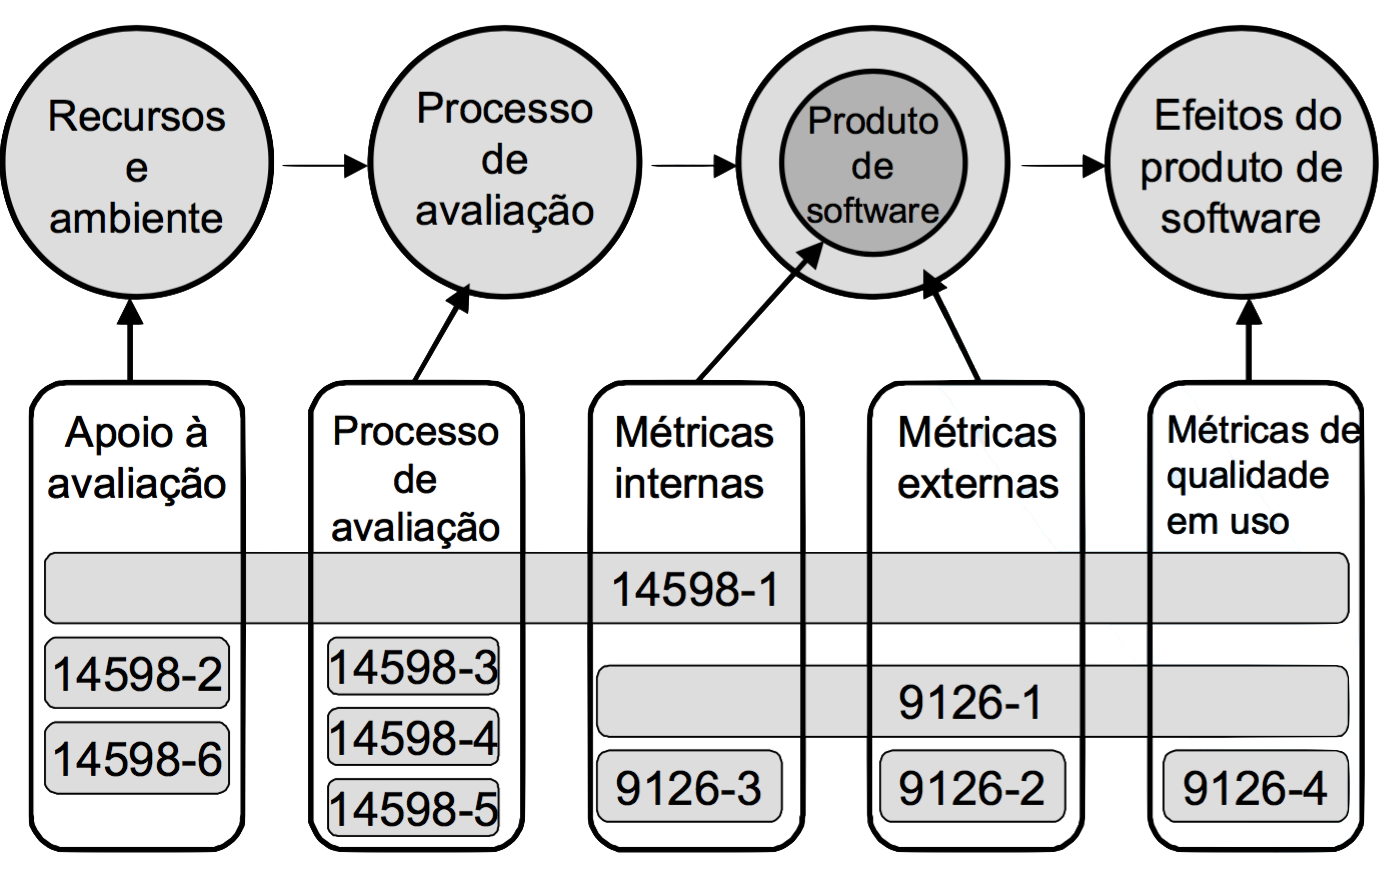
\includegraphics[scale=0.40]{ISO}
\caption{Relação entre as NBR ISO/IEC 9126 e NBR ISO/IEC 14598 .Fonte:\cite{_nbr_2016}}
\label{img:relacao_iso}
\end{figure}

Como modelo de qualidade,a ISO 9126 classifica a qualidade interna do produto como sendo o somatório das características do ponto de vista interno do software. Os principais produtos desta categoria são os de cunho intermediário, entre eles: relatórios de análise estática do código fonte, revisão dos documentos produzidos, entre outros. A qualidade externa, por sua vez, já apresenta foco mais voltado para as relações externas do software, normalmente, relacionando-se com a execução do código. Nesse caso, é necessário coletar suas métricas, enquanto o software está em funcionamento. A Figura \ref{img:modelo_qualidade} apresenta a divisão proposta pela \cite{_nbr_2016}, onde são categorizados seis aspectos de qualidade de software e suas sub características, medidas por meio de métricas internas e externas.
\graphicspath{{figuras/}}
\begin{figure}[h]
\centering
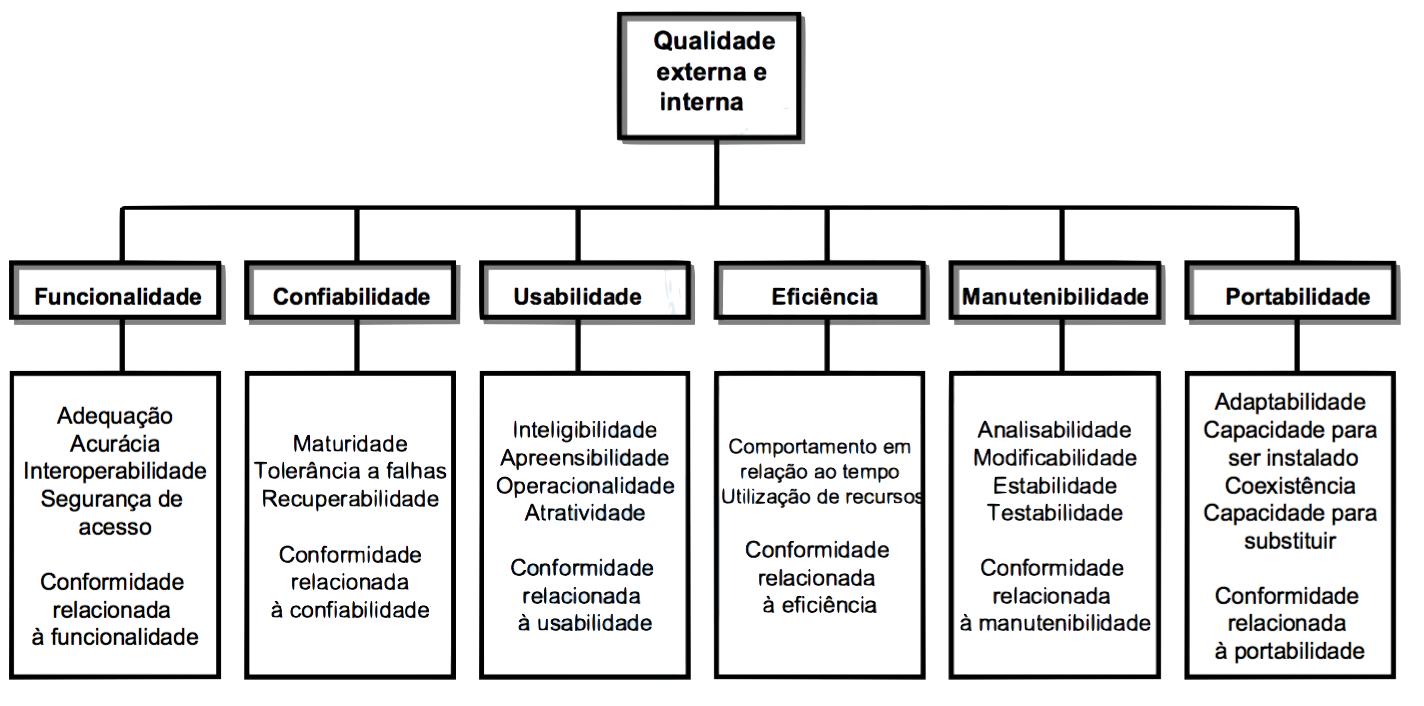
\includegraphics[scale=0.50]{Modelo_de_Qualidade}
\caption{Modelo de Qualidade para Qualidade Interna e Externa .Fonte:\cite{_nbr_2016}}
\label{img:modelo_qualidade}
\end{figure}

Segundo a ISO 9126, essas características podem ser definidas como:
\begin{itemize}
\item \textbf{Funcionalidade}: Capacidade do produto de software de prover funções que atendam às necessidades explícitas e implícitas, quando o software estiver sendo utilizado sob condições especificadas.
\item \textbf{Confiabilidade}:Capacidade do produto de software de manter um nível de desempenho especificado, quando usado em condições especificadas.
\item \textbf{Usabilidade}: Capacidade do produto de software de ser compreendido, aprendido, operado e atraente ao usuário, quando usado sob condições especificadas.
\item \textbf{Eficiência}: Capacidade do produto de software de apresentar desempenho apropriado, relativo à quantidade de recursos usados, sob condições especificadas.
\item \textbf{Manutenibilidade}: Capacidade do produto de software de ser modificado. As modificações podem incluir correções, melhorias ou adaptações do software devido a mudanças no ambiente e nos seus requisitos ou especificações funcionais.
\item \textbf{Portabilidade}: Capacidade do produto de software de ser transferido de um ambiente para outro.
\end{itemize}

Em 2011, surgiu um conjunto de normas conhecido como SQuaRE. Esse conjunto trazia um \textit{framework} aprimorado à atual norma vigente. Além disso, tinha como objetivo avaliar o produto de qualidade de software.

\subsection{Norma SQuaRE}
O conjunto de normas SQuaRE (Requisitos e Avaliação de Qualidade de Sistema e Software) surgiu para substituir a ISO/IEC 9126. O objetivo destas normas é prover um \textit{framework} que avalie a qualidade do produto de software \cite{luiza_yago}. ISO/IEC 25010 mantém as características de qualidade já definidas na ISO 9126 com alguns incrementos.

\begin{itemize}
\item O escopo dos modelos de qualidade foram estendidos para incluir sistemas computacionais e a qualidade em uso sob o ponto de vista do sistema.
\item Segurança foi adicionada como característica, e não uma sub-característica de funcionalidade.
\item Compatibilidade foi adicionada como característica.
\item A qualidade interna e externa foram combinadas como modelo de qualidade de produto.
\end{itemize}

A norma apresenta três guias de qualidade. O primeiro modelo é referente à Qualidade do Produto; o segundo, à Qualidade em Uso, e o último, à Qualidade de Dados.O modelo de Qualidade do Produto subdivide um sistema de software em oito categorias, como mostra a Figura \ref{img:modelo_square}.
Assim como a ISO 9126, a ISO 25010 também apresenta categorias, estas categorias assemelham-se às categorias da ISO 9126, sendo essa base para criação da norma SQuaRE. Seguem as características:

\begin{itemize}
\item \textbf{Adequação Funcional}: nível que determina o quanto um produto ou sistema satisfazem as especificações providas pelo usuário.
\item \textbf{Eficiência de Desempenho}: desempenho relativo à quantidade de recursos usados em condições específicas.
\item \textbf{Compatibilidade}: o nível que um sistema ou produto pode compartilhar informações, com outros produtos, sistemas ou componentes.
\item \textbf{Usabilidade}: O nível que um produto ou sistema pode ser usado por usuários específicos para atingir seus objetivos com efetividade, eficiência e satisfação em contexto específico de uso.
\item \textbf{Confiabilidade}: nível que um sistema, produto ou componente executa suas atividades em um contexto pré-determinado e específico para uso.
\item \textbf{Segurança}: nível no qual um sistema protege as informações e os dados de maneira que pessoas ou outros sistemas tenham acesso limitado de acordo com nível de autorização específico.
\item \textbf{Manutenibilidade}: nível de efetividade e eficiência, com o qual um produto ou sistema pode ser modificado pelos sistemas mantenedores.
\item \textbf{Portabilidade}: Nível de efetividade e eficiência com o qual um sistema, produto ou componente pode ser transferido de um \textit{hardware}, software ou ambiente de uso para outro.
\end{itemize}
\graphicspath{{figuras/}}
\begin{figure}[h!]
\centering
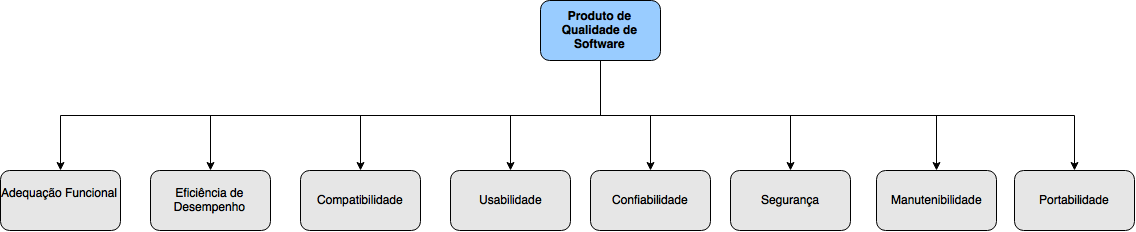
\includegraphics[scale=0.40]{SQuaRE}
\caption{Produto de Qualidade de Software.Fonte:\cite{Square}}
\label{img:modelo_square}
\end{figure}

Este trabalho tem seu desenvolvimento focado no modelo de Qualidade de Uso
o qual apresenta características externas ao software, e os resultados sendo coletados através de atributos estáticos \cite{Square}. O foco deste trabalho está em medir indicadores quanto à manutenibilidade do software. Essa característica está diretamente ligada ao processo de Manutenção do Software.

\subsection{Manutenção de Software}
Segundo Sommervile \cite{sommervile}, manutenção de software é o processo de alterar o sistema depois que ele foi publicado. As alterações feitas no software podem ser simples correções de erro, até mudanças significativamente grandes, falhas arquiteturais, ou mesmo melhorias para acomodar novos requisitos.

Outra visão sobre manutenção de software é dada por Pressman \cite{pressman}, em que o autor conceitua o termo como sendo a correção de defeitos, e adaptação do software para lidar com uma mudança do ambiente e aperfeiçoar as funcionalidades em atendimento às necessidades dos usuários. Outra característica do processo de manutenção é a sua composição por um conjunto de subprocessos, atividades e tarefas que podem ser utilizados durante a fase de manutenção para alterar um produto de software, contanto que seja mantido o seu funcionamento \cite{calazans_avaliacao_2005}.

Para Sommervile, existem quatro categorias de manutenção:
\begin{itemize}
\item \textbf{Manutenção Corretiva}: seu objetivo está em identificar e remover falhas de software
\item \textbf{Manutenção Adaptativa}: provê modificações no software para alojar mudanças no ambiente externo. Nesta manutenção, também está incluso o processo de migração para diferentes plataformas tanto de software quanto de \textit{hardware}.
\item \textbf{Manutenção Perfectiva}: feita com o intuito de aperfeiçoar o software, além dos requisitos funcionais originais. Esta expansão dos requisitos traz consigo uma melhoria às funcionalidades até então implementadas ou um ganho de desempenho do sistema.
\item \textbf{Manutenção Preventiva}: implementada para permitir que seja mais simples a correção, adaptação ou melhoria do software.
\end{itemize}

O modelo da Figura \ref{img:modelo_manutencao} apresenta as atividades propostas por Pfleeger \cite{pfleeger_framework_1990} para um processo de manutenção. Na figura, percebe-se que o processo de acompanhamento da manutenção ocorre durante todo o processo. As atividades apresentadas no diagrama são:

\begin{itemize}
\item \textbf{Análise do Impacto da Mudança de Software}: estima o impacto de uma determinada mudança. Nesta atividade, determina-se o grau de mudança e o quanto esta mudança impactará no resto do software. 
\item \textbf{Entendimento do Software a ser Alterado}: nesta atividade, são analisados os códigos-fonte do software para entender a mudança e a integração do que deve ser alterado. Esta atividade depende muito do grau de manutenibilidade do software, uma vez que quanto mais manutenível, mais fácil e rápido se dá o processo de análise do software.
\item \textbf{Implementação da Mudança}: incremento ou modificação do software. Esta atividade é diretamente relacionada com o grau de adaptação do software; o quanto o software pode ser expandido ou comprimido. Essa característica de adaptabilidade é uma sub-característica da manutenibilidade de software apresentada pela norma SQUARE. 
\item \textbf{Mudanças pelo Efeito Cascata}: Análise da propagação das mudanças ao longo do software. Essa atividade está intimamente relacionada ao indicador de coesão, que relaciona a responsabilidade de uma classe com seus métodos, e acoplamento do software, este afere o quão amarrado estão as classes e os métodos do software.
\item \textbf{(Re)Teste do Software}: é a última atividade antes da entrega do software alterado. O software é testado novamente sob a perspectiva do novo requisito.
\end{itemize}

\graphicspath{{figuras/}}
\begin{figure}[h!]
\centering
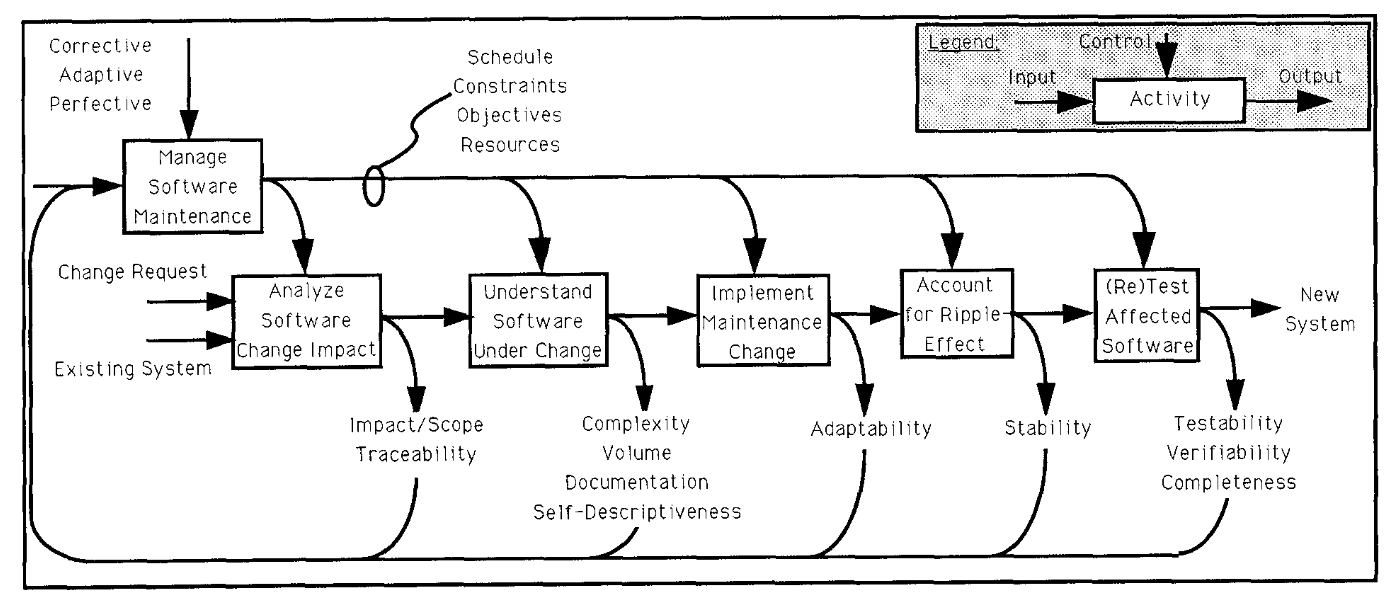
\includegraphics[scale=0.50]{Manutencao}
\caption{Diagrama das Atividades de Manutenção de Software.Fonte:\cite{pfleeger_framework_1990}}
\label{img:modelo_manutencao}
\end{figure}

Um estudo realizado por Kustyers e Heemstra \cite{kusters} mostra as dificuldades atuais na manutenção de software com base em seis grandes organizações da Alemanha. Um dos resultados obtidos foi que existe um uma falta muito grande na percepção quanto ao tamanho e ao custo das manutenções de software. Os autores relatam que os gastos com manutenção são altos, e que das seis empresas apenas uma guardava os registros  dos seus processos de manutenção, e os usava para fazer um novo planejamento. 

Normalmente, tem se como verdade, de que a manutenção de software está unicamente ligada ao conserto de \textit{bugs}. Entretanto, estudos e \textit{surveys} ao longo dos anos comprovam que mais de 80\% do esforço gasto na manutenção é utilizado em ações não corretivas, segundo Pigosky \cite{pigosky}. O autor também afirma que entre 40\% a 60\% do esforço de manutenção está em entender o software que será modificado.

\section{Métricas de Qualidade de Software}

Uma métrica é uma função que pode ser medida. Métrica de qualidade de software é uma função; cuja entrada é uma informação de software, e cuja saída é um único valor numérico que pode ser interpretado como o nível que é dado a um software \cite{karner}. Segundo \cite{pressman}, métricas podem ser definidas como sendo um pequeno subconjunto de informações úteis acerca do software.

Segundo Mills, algumas características são inerentes a uma boa métrica, tais como, simplicidade, objetividade, fácil obtenção, validade, robustez, linearidade de escala. Diversos autores sugeriram conjunto de métricas que combinadas tratam de várias áreas de qualidade de software \cite{paulo_meirelles}.

A ferramenta SonarQube apresenta algumas métricas dentre as quais ressalta-se:

\begin{itemize}
\item\textbf{Complexidade} = é a complexidade baseada no número de caminhos pelo código. Sempre que o fluxo de um caminho se divide, o contador da complexidade é incrementado em 1. Toda função tem no mínimo complexidade igual a 1.
\item\textbf{Complexidade por Classe} = média aritmética da complexidade em todas as classes.
\item\textbf{Linhas Comentadas} = número de linhas que contém comentários fazem parte de um bloco de comentários. Linhas de comentário não significativas (linhas vazias ou que possuam apenas caracteres especiais), não incrementam o número de linhas comentadas.
\item\textbf{\% Comentários} = Definido como sendo a densidade de linhas de código comentadas, é calculada como sendo o número de linhas comentadas / número de linhas totais.

%( \frac{Linhas Comentadas}{Total de Linhas} ) * 100

\item\textbf{Linhas Duplicadas \%} = densidade do número de blocos de linhas duplicados.

%( \frac{Linhas Duplicadas}{Total de Linhas} ) * 100

\item\textbf{\textit{Issues}} = Erros de código. Podem ser classificados quanto a sua severidade como sendo:
\begin{itemize}
\item\textbf{\textit{Blocker}} = risco operacional ou de segurança. Este tipo de \textit{issue} pode tornar toda a aplicação instável quando estiver no ambiente de produção. Ex: calling garbage collector, not closing a socket, etc.
\item\textbf{\textit{Critical}} = risco operacional ou de segurança. Este tipo de \textit{issue} pode levar a um comportamento inesperado quando em produção, sem impactar a integridade de toda a aplicação. Ex: NullPointerException, badly caught exceptions, lack of unit tests, etc.
\item\textbf{\textit{Major}} = este tipo de \textit{issue} pode ter um impacto substancial na aplicação. Ex: too complex methods, package cycles, etc.
\item\textbf{\textit{Minor}} = esta \textit{issue} pode impactar de maneira mínima ou substancial a aplicação. Ex: naming conventions, Finalizer does nothing but call superclass finalizer, etc.
\item\textbf{Info} = não conhecidos ou não foram definidos impactos na aplicação.
\end{itemize}

\item\textbf{Débito Técnico} = esforço gasto para consertar todas as \textit{issues}. A medida é feita de forma que um dia possua 8 horas. Logo, caso o valor encontrado seja maior do que 8 horas, o sistema irá mostrar o resultado em dias.

\item\textbf{Relação do Débito Técnico Com O Custo} = (\textit{Technical Debt Ratio} ou TDR) relação entre o custo de desenvolvimento do software e o custo para conserta-lo. O custo de produção é definido como sendo 1 linha de código para 0.06 dias.

\[\frac{Custo de Conserto}{Custo de Produção}\]

\item\textbf{Índice de Manutenibilidade} = também conhecido como Índice SQALE, é dado a um projeto relacionando-o com o valor do TDR. A escala  padrão do Índice de Manutenibilidade é: 
\begin{itemize}
\item[A] 0-0.5
\item[B] 0.06-0.1
\item[C] 0.11-0.20
\item[D] 0.21-0.5
\item[E] 0.5-1
\end{itemize}

\item\textbf{Número de Linhas} = número de linhas que contém pelo menos um carácter que não seja espaço em branco, tabulação ou parte de um comentário.

\end{itemize}

Outra ferramenta muito utilizada para fazer análise estática de código é o Codacy. O Codacy diferencia-se do Sonarqube devido ao fato de ele não ser \textit{Open Source} e ser totalmente \textit{online}, enquanto o Sonarqube é \textit{Open Source} e funciona de maneira offline. Algumas das métricas apresentadas pelo Codacy são: 

\begin{itemize}
\item\textbf{Estilo de Código} =  formatação de código e problemas de sintaxe. Ex: estilo de nome de variáveis, uso de chaves e aspas para marcação.
\item\textbf{\textit{Error Prone}} = código que pode esconder \textit{bugs} e palavras chaves da linguagem que deveriam ser usadas com cuidado. Ex: == em Java ou Option.get em Scala.
\item\textbf{\textit{Performance}} = código que pode afetar a performance da aplicação.
\item\textbf{Compatibilidade} = usado primariamente para código \textit{front-end}, detecta problemas de compatibilidade de versão entre diferentes versões de \textit{browsers}.
\item\textbf{Código não Utilizado} = variáveis e métodos não utilizados.
\item\textbf{Segurança} = problemas de segurança.
\item\textbf{Documentação} = detecta métodos e classes que não possuem a documentação da maneira correta.

\end{itemize}

Devido ao conjunto de métricas ser vasto e pouco conhecido por meio dos gestores, uma das soluções encontradas está na utilização de aprendizado de máquina para sugerir possíveis métricas.


\section{Aprendizado de Máquina e Sistemas de Recomendação}

Aprendizado de Máquina se caracteriza pela implementação de técnicas que ajudam a melhorar o desempenho de um software aprendendendo através de conhecimento indutivo \cite{mitchell1997mcgraw}. Maria Carolina \cite{monard2003conceitos} diz "A indução é a forma de inferência lógica que permite obter conclusões genéricas sobre um conjunto particular de exemplos. Ela é caracterizada como o raciocínio que se origina em um conceito específico e o generaliza, ou seja, da parte para o todo. Na indução, um conceito é aprendido efetuando-se inferência indutiva sobre os exemplos apresentado". Esse conhecimento se baseia no conceito que modelos são obtidos através de um conjunto de dados ou representações de experiências \cite{peres2012tutorial}. Podem ser divididos em duas categorias: aprendizagem supervisionada e não supervisionada \cite{russell2009artificial}.
\begin{itemize}
\item\textbf{Aprendizagem Supervisionada:} o algoritmo recebe dados exemplos de entradas e de saída e com base nesses exemplos define uma regra.
\item\textbf{Aprendizagem Não Supervisionada: } o algoritmo recebe apenas dados de entrada e o próprio algoritmo define os conjuntos e as saídas desses conjuntos.
\end{itemize}

Para que seja possível o aprendizado de máquina são necessários algoritmos que irão conduzir esse aprendizado. Um dos algoritmos é o por análise de agrupamento \textit{clustering}. Esse algoritmo serve para agrupar um conjunto de objetos de forma que os objetos que sejam mais semelhantes estejam no mesmo grupo (\textit{cluster}). Algumas das formas de se fazer esse agrupamento são utilizando a distância entre os pontos, aproximação por centróides entre outras.

Segundo Lucas \cite{brunialti2015aprendizado} um Sistema de Recomendação (SR)tem por objetivo principal sugerir itens que possam satisfazer a necessidade de um usuário sob um determinado aspecto. No livro \textit{"Recommender systems: an introduction"} \cite{jannach2010recommender} são apresentados modelos de SR que se caracterizam pela forma como o SR é implementado. O primeiro modelo é o colaborativo, neste modelo as recomendações são feitas através de itens que os usuários interagiram no passado e relacionando essas informações. A figura \ref{img:sr1} apresenta um exemplo de SR por recomendação em que o item "laranja" é recomendado para o usuário 3 pelo fato de que tanto o usuário 1 quanto ao usuário 3 compraram "maçã", nesta lógica se o usuário 1 comprou "laranja" o usuário 3 também pode querer maçã. 

\graphicspath{{figuras/}}
\begin{figure}[h!]
\centering
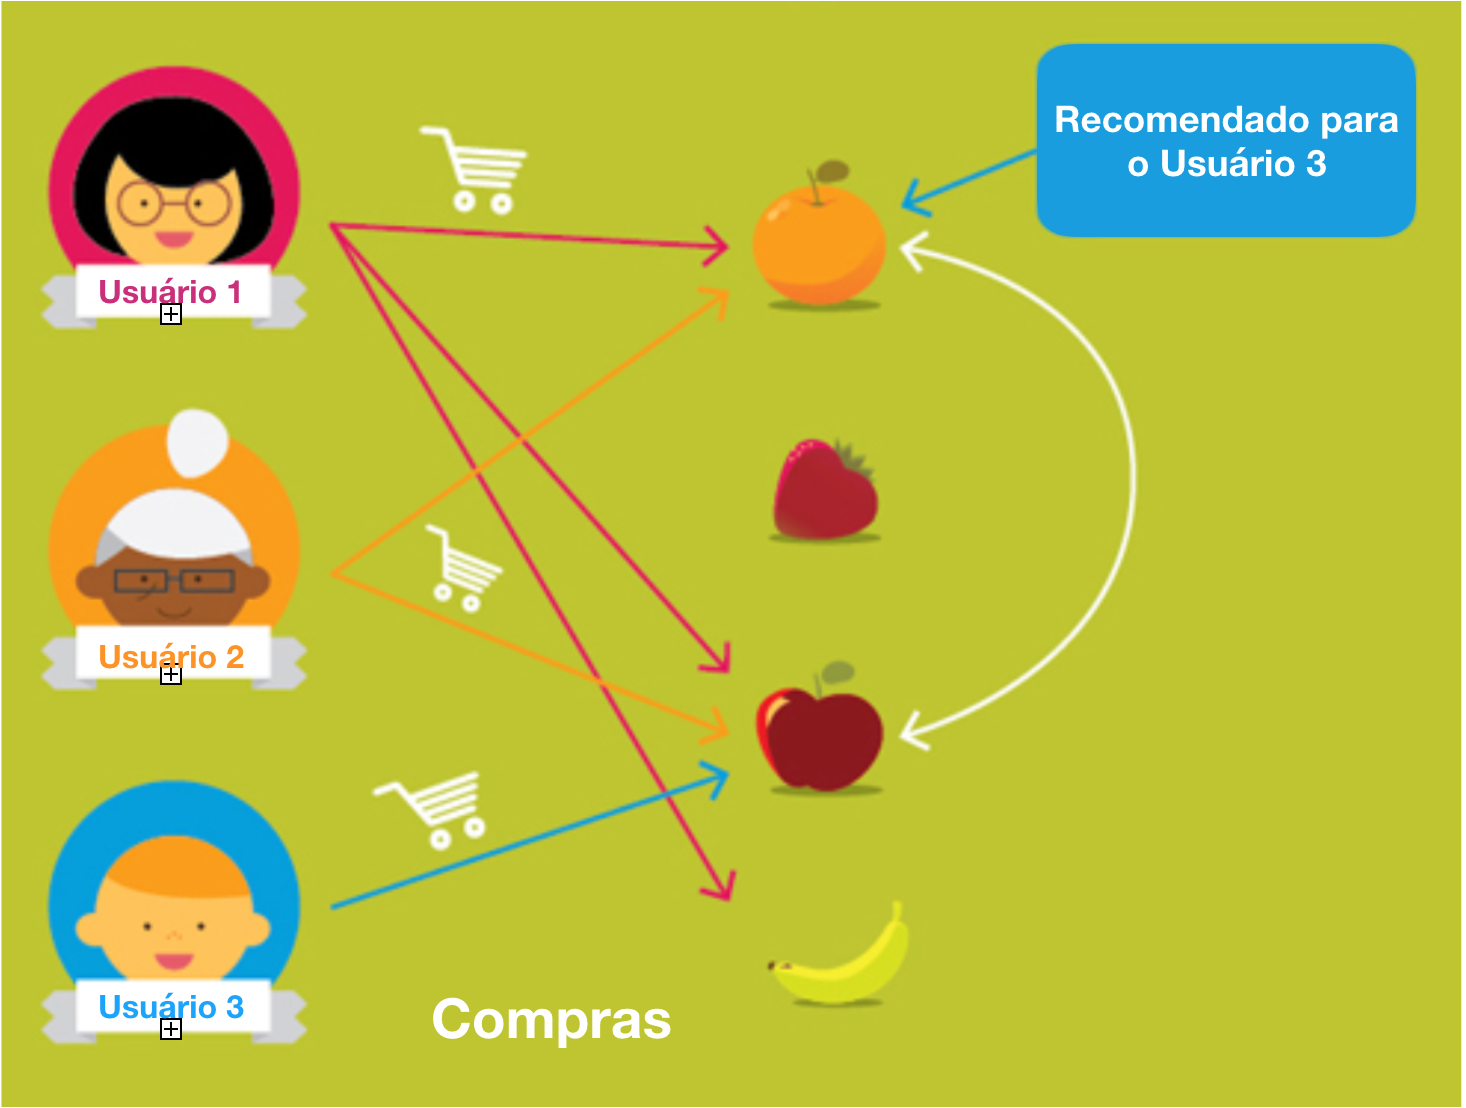
\includegraphics[scale=0.50]{sr1.png}
\caption{SR por Colaboração. Adaptado de: \cite{sarwar2001item}}
\label{img:sr1}
\end{figure}

O segundo modelo é o com base no conteúdo, onde as recomendações são obtidas através das características dos itens e no perfil do usuário. Uma analogia pode ser feita da seguinte maneira.

 \begin{itemize}
 \item SR baseado em um \textbf{Sistema Colaborativo}: "Usuários que são similares a você também gostaram ..."
 \item SR baseado em um \textbf{Sistema de Conteúdo}: "Usuários que gostaram desse item também gostaram ..." 
 \end{itemize}
 

Baseando em um SR que utiliza Sistema de Conteúdo, A fórmula Euclidiana apresenta a menor distância entre dois pontos, neste caso a menor distância representa o grau de similaridade entre dois usuários. 

\[E(x,y) = \sqrt{\sum_{i=0}^{n}(xi-yi)^{2}}\]


Uma vez que as métricas se encontram definidas, deve-se pensar na melhor maneira de exibir as métricas para o usuário. O papel da visualização das métricas de software é definir, com base na natureza, e na escala de uma métrica, qual a melhor maneira de imprimir na tela essas informações.


\section{Visualização da Informação}
Computadores tornaram-se peças fundamentais do cotidiano do ser humano do século 21. Seja para lazer, estudo, comunicação, o computador revolucionou significamente em cada área que passou \cite{hasan_humancomputer_2014}.
A visualização de software pode ser definida como uma disciplina que faz uso de várias formas de imagens que servem de insumo para compreender, entender e reduzir a complexidade dos sistemas de software existentes \cite{gracanin_software_2005}. Porém, a visão que melhor se adapta ao contexto deste trabalho é dada por Gomes \cite{gomes_percepcao_2011}, que diz que a visualização de uma forma generalizada é a construção de uma imagem visual na mente humana, e está imagem vai além de representações gráficas ou conceitos.

Uma vez que são coletados os dados, esses já estão categorizados de acordo com a sua natureza, e podem ser exibidos. Mas, ainda é necessário discutir qual a melhor forma de exibir  todas essas informações na tela. Uma das formas de se agrupar toda a informação de maneira ordenada e com sentido lógico é através de \textit{dashboards} \cite{book_design}. O conceito será apresentado no tópico a seguir.


\subsection{Dashboard}
O conceito apresentado por Stephen Few em seu livro \cite{book_design}, diz que um \textit{dashboard} é um \textit{display} virtual das informações mais importantes para atingir um ou mais objetivos. Deve ser construído e organizado para ser capaz de caber em uma única página para que a informação seja achada com facilidade. Esta seção visa apresentar alguns modelos de \textit{dashboards} e suas características.

Schwendimann \cite{schwendimann_perceiving_2016} apresenta uma revisão sistemática sobre \textit{dashboard} para aprendizado. A pesquisa foi feita em 55 artigos. Na Figura \ref{img:tipo_visualizacao} pode-se ver que os três tipos de visualização mais utilizados são gráfico de barras (33 artigos), gráfico de linhas (24 artigos) e tabelas (21 artigos).
\graphicspath{{figuras/}}
\begin{figure}[h!]
\centering
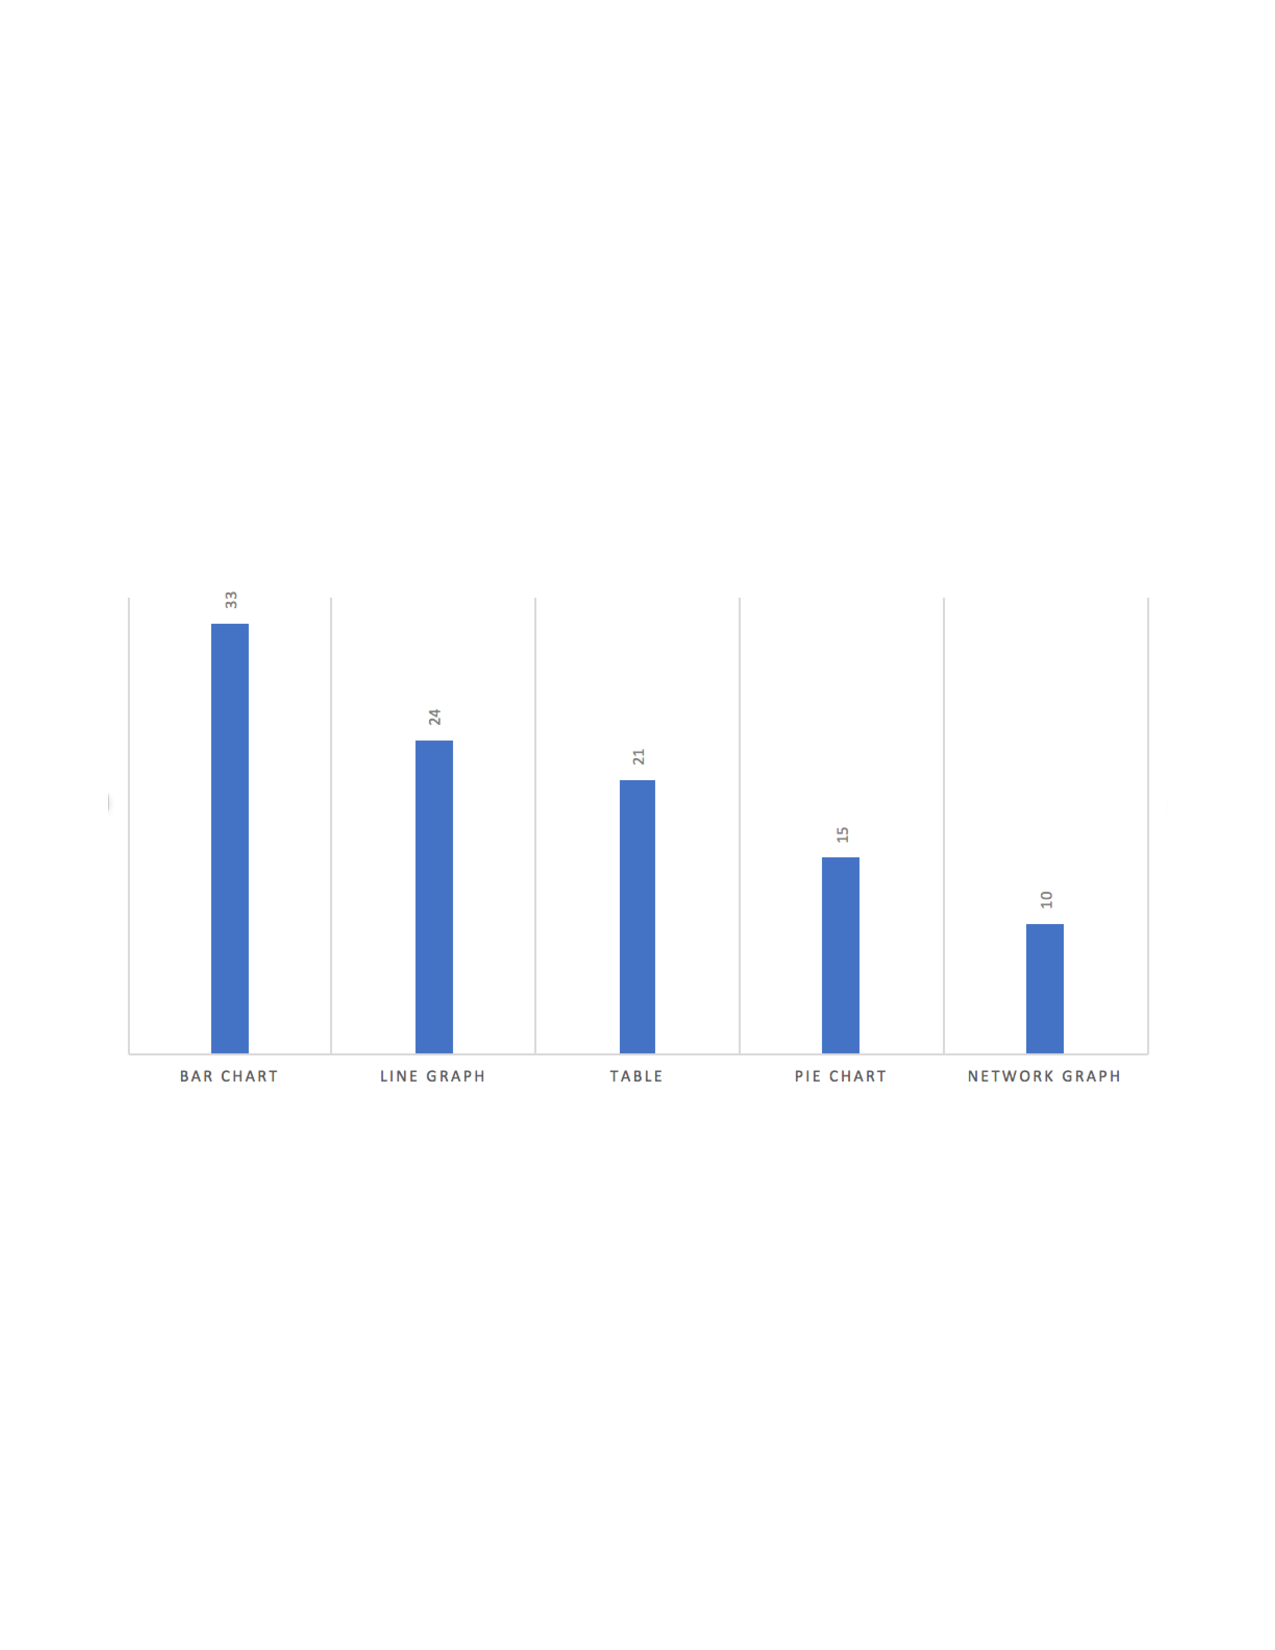
\includegraphics[scale=0.60]{grafico_pesquisa}
\caption{Tipos de Visualização Mais Frequente. Fonte: \cite{schwendimann_perceiving_2016}}
\label{img:tipo_visualizacao}
\end{figure}

\begin{itemize}

\item Gráfico de Barras: representação de quantidade ao longo de uma escala numérica (Figura \ref{img:bar_graph}). Para que haja uma comparação significativa, deve ser feita sob a perspectiva de uma escala linear, partindo de zero\cite{doumont_choosing_2002}
\graphicspath{{figuras/}}
\begin{figure}[H]
\centering
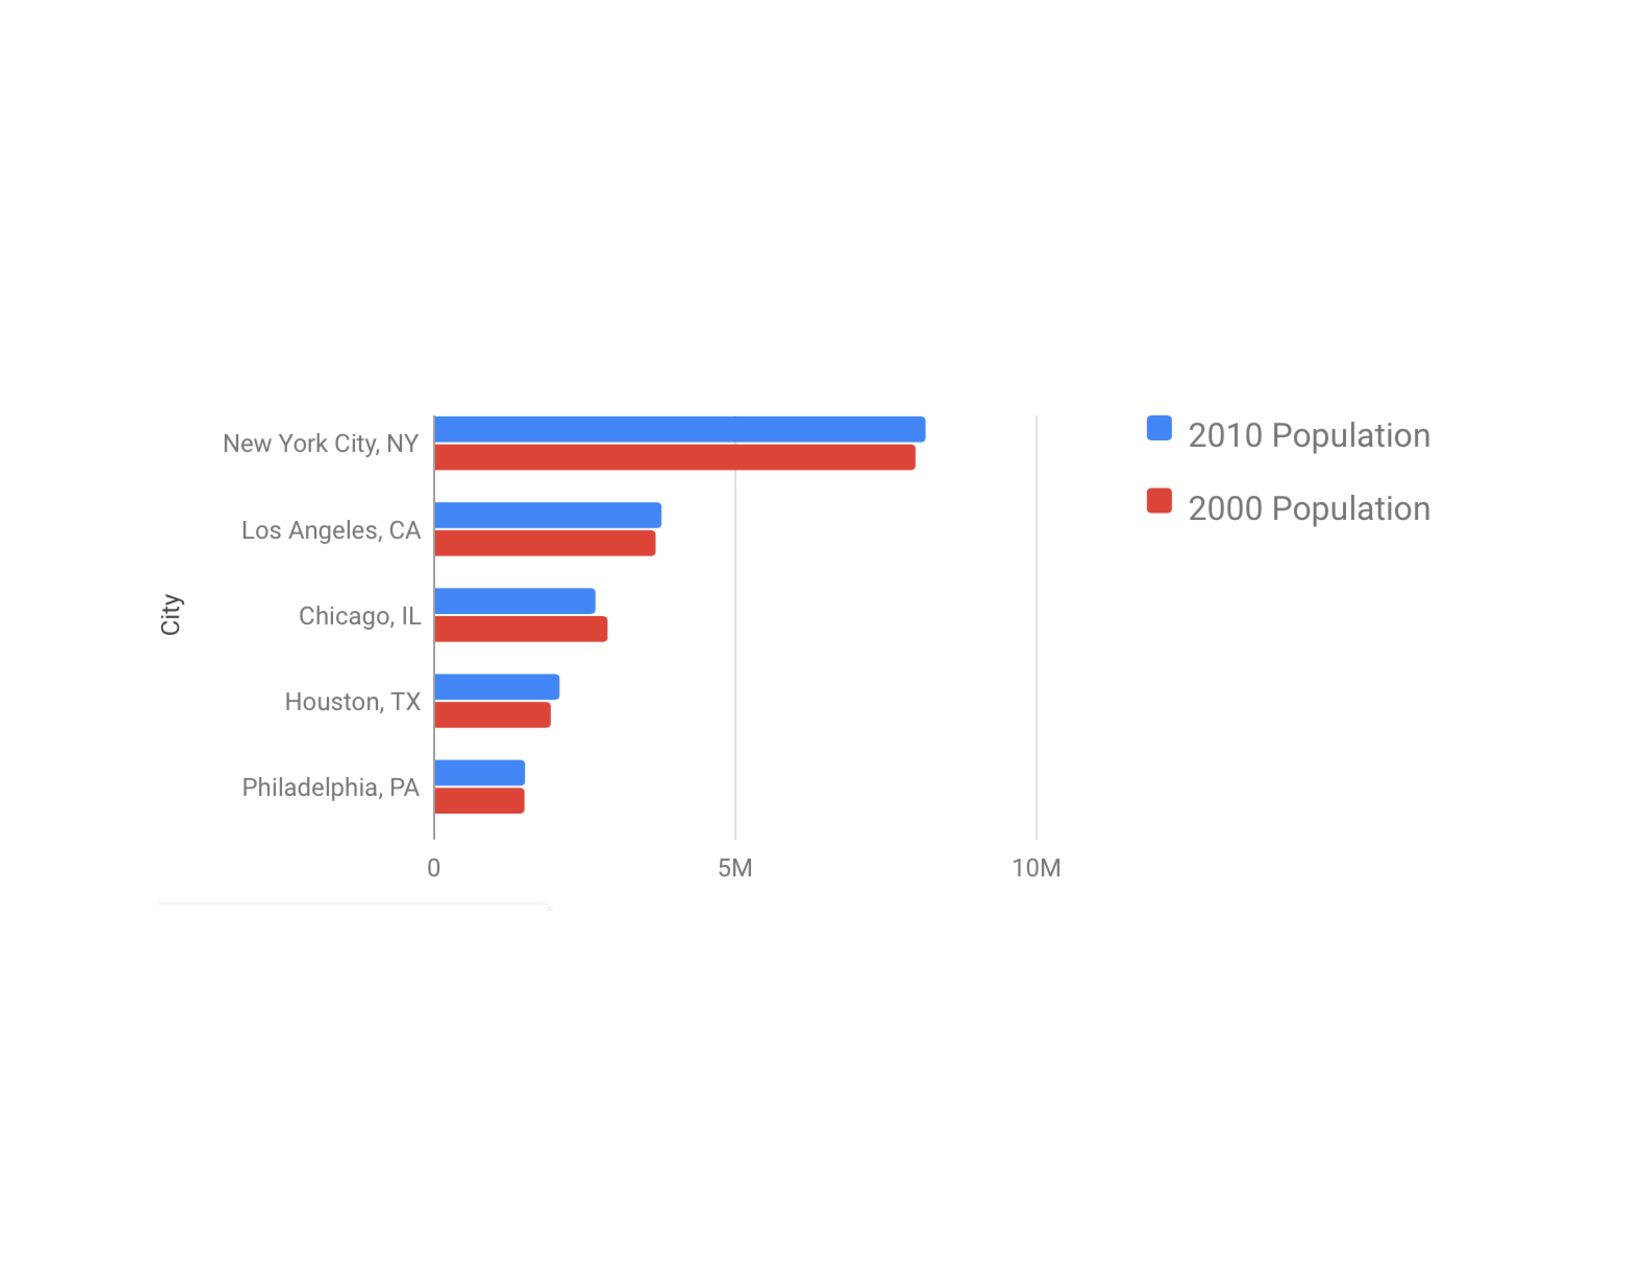
\includegraphics[scale=0.40]{chart_bar}
\caption{Exemplo de Gráfico de Barra Utilizando Google Charts}
\label{img:bar_graph}
\end{figure}

\item Gráfico de Linhas: muito utilizado quando se tem um conjunto de dados contínuos. Pode ainda ser utilizado para determinar padrões ou uma tendência (Figura \ref{img:line_graph}). Normalmente, representam dados relacionados à tempo.
\graphicspath{{figuras/}}
\begin{figure}[H]
\centering
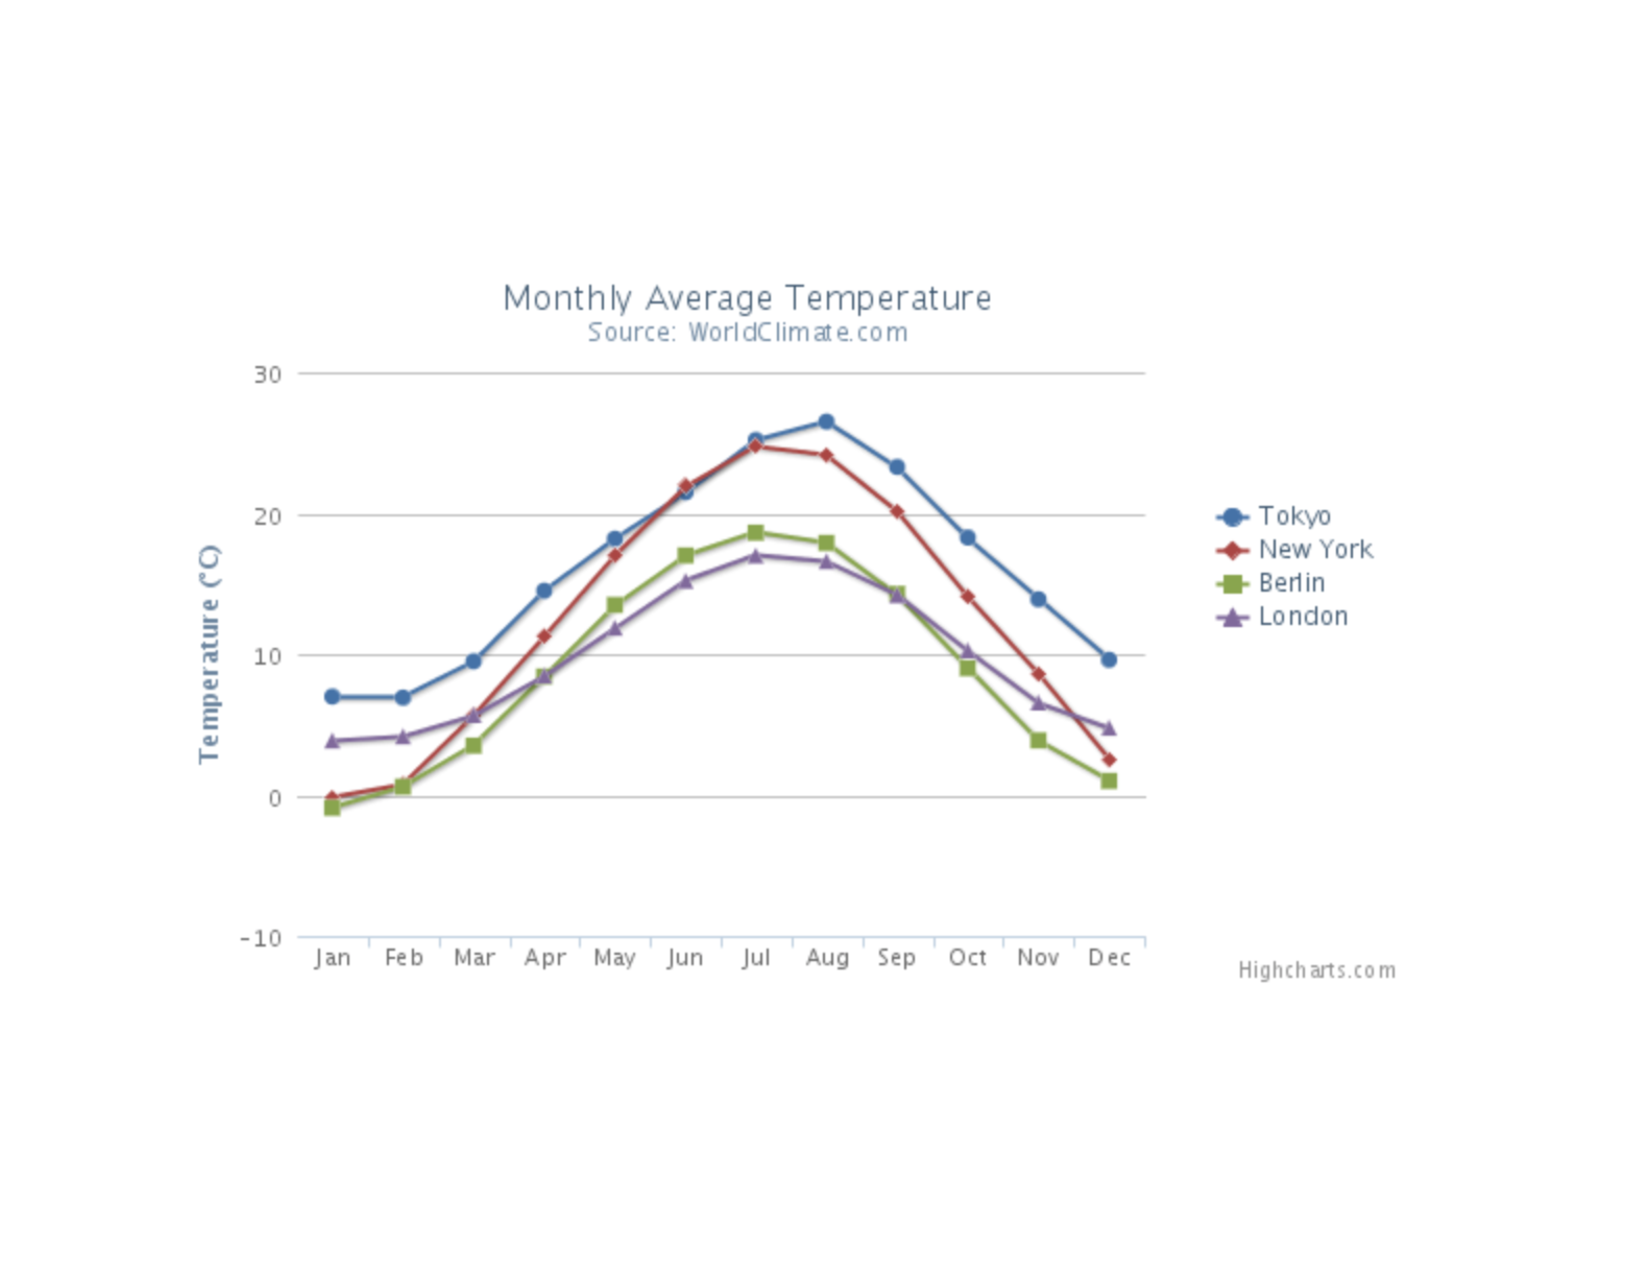
\includegraphics[scale=0.40]{line_chart}
\caption{Exemplo de Gráfico de Linhas utilizando HiCharts}
\label{img:line_graph}
\end{figure}

\item Gráfico de Pizza: é melhor usado quando se deseja comparar um setor em relação ao total. O gráfico de pizza é um gráfico circular dividido em segmentos. Cada segmento representa uma categoria e o somatório dessas partes formam o todo (Figura \ref{img:pie_chart}). Não se aconselha utilizar o gráfico de pizza quando se tem que representar mais de sete categorias.
\graphicspath{{figuras/}}
\begin{figure}[H]
\centering
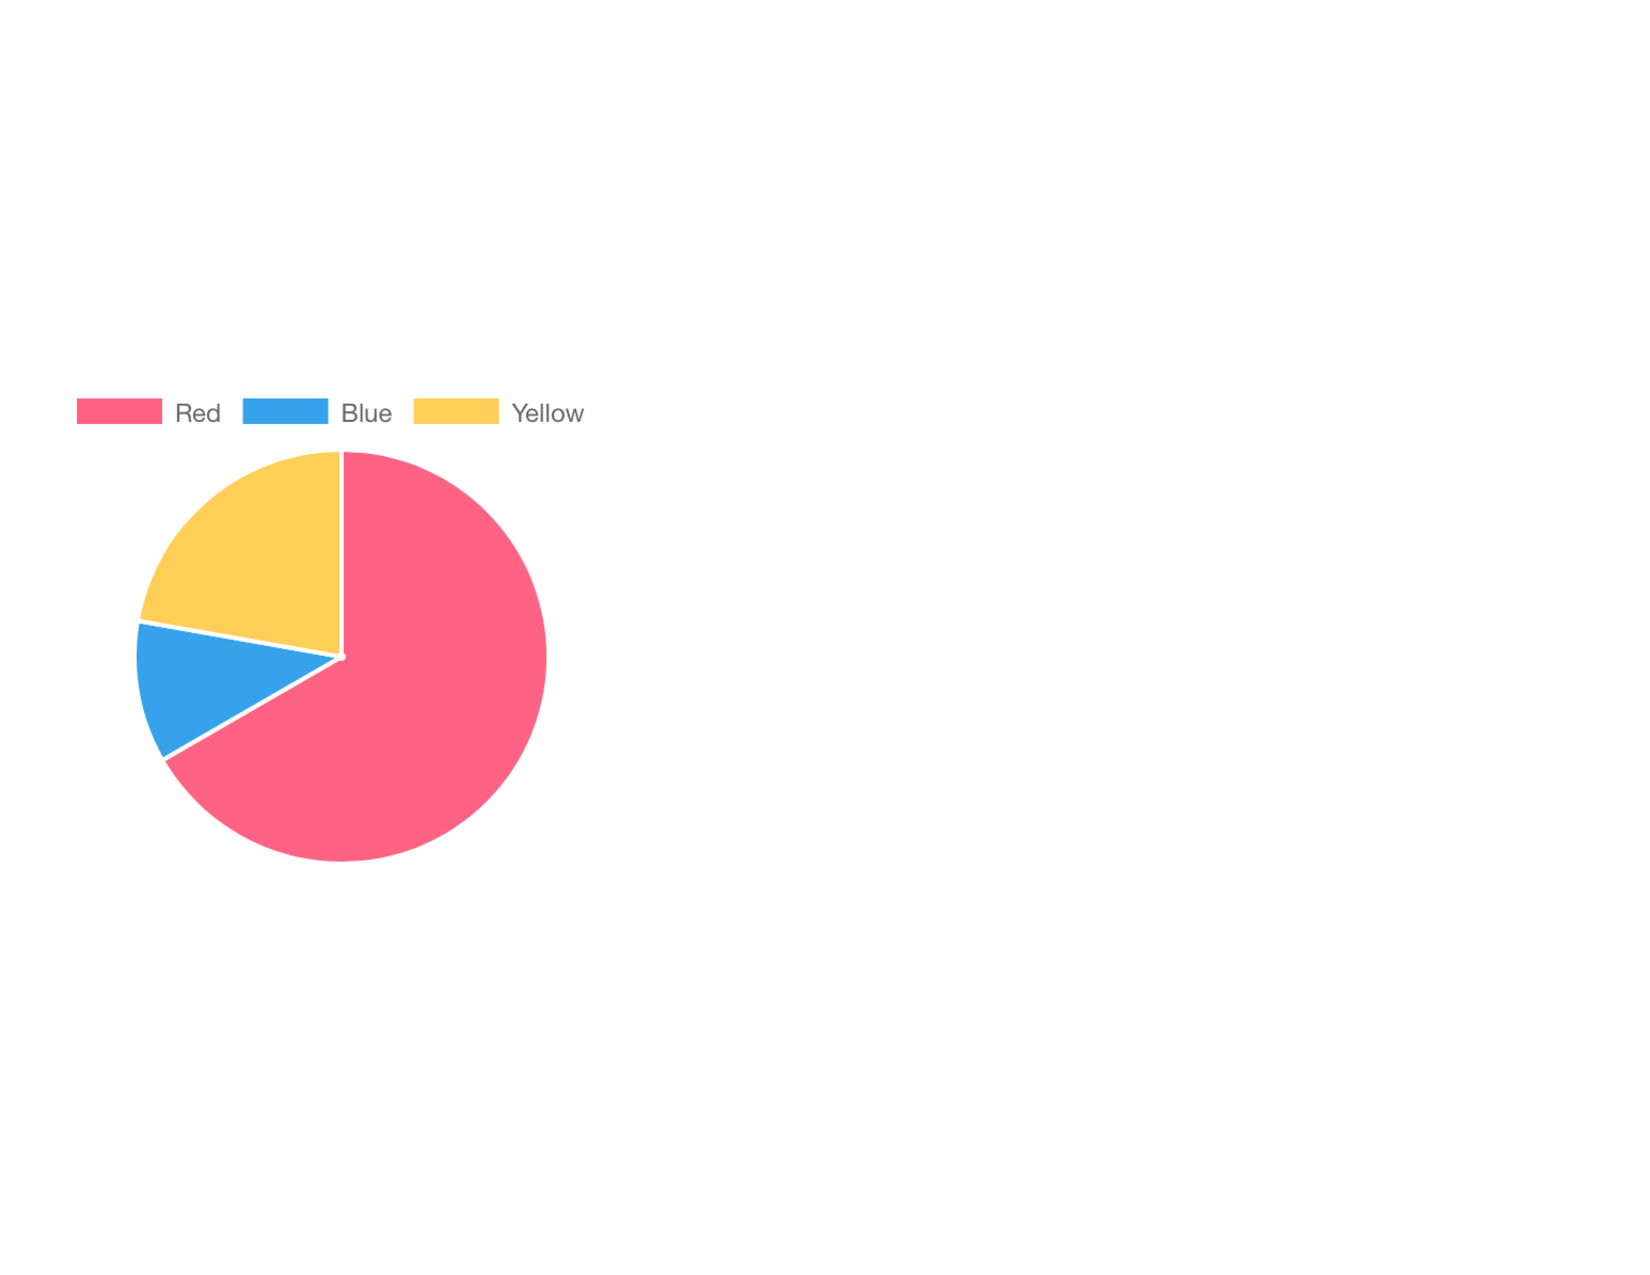
\includegraphics[scale=0.40]{pie_chart}
\caption{Exemplo de Gráfico de Pizza utilizando Chart.js}
\label{img:pie_chart}
\end{figure}

\item \textit{Network Chart}: este tipo de visualização reforça relacionamentos entre entidades. As entidades são mostradas como nós e os relacionamentos como linhas (Figura \ref{img:network_graph}).
\graphicspath{{figuras/}}
\begin{figure}[H]
\centering
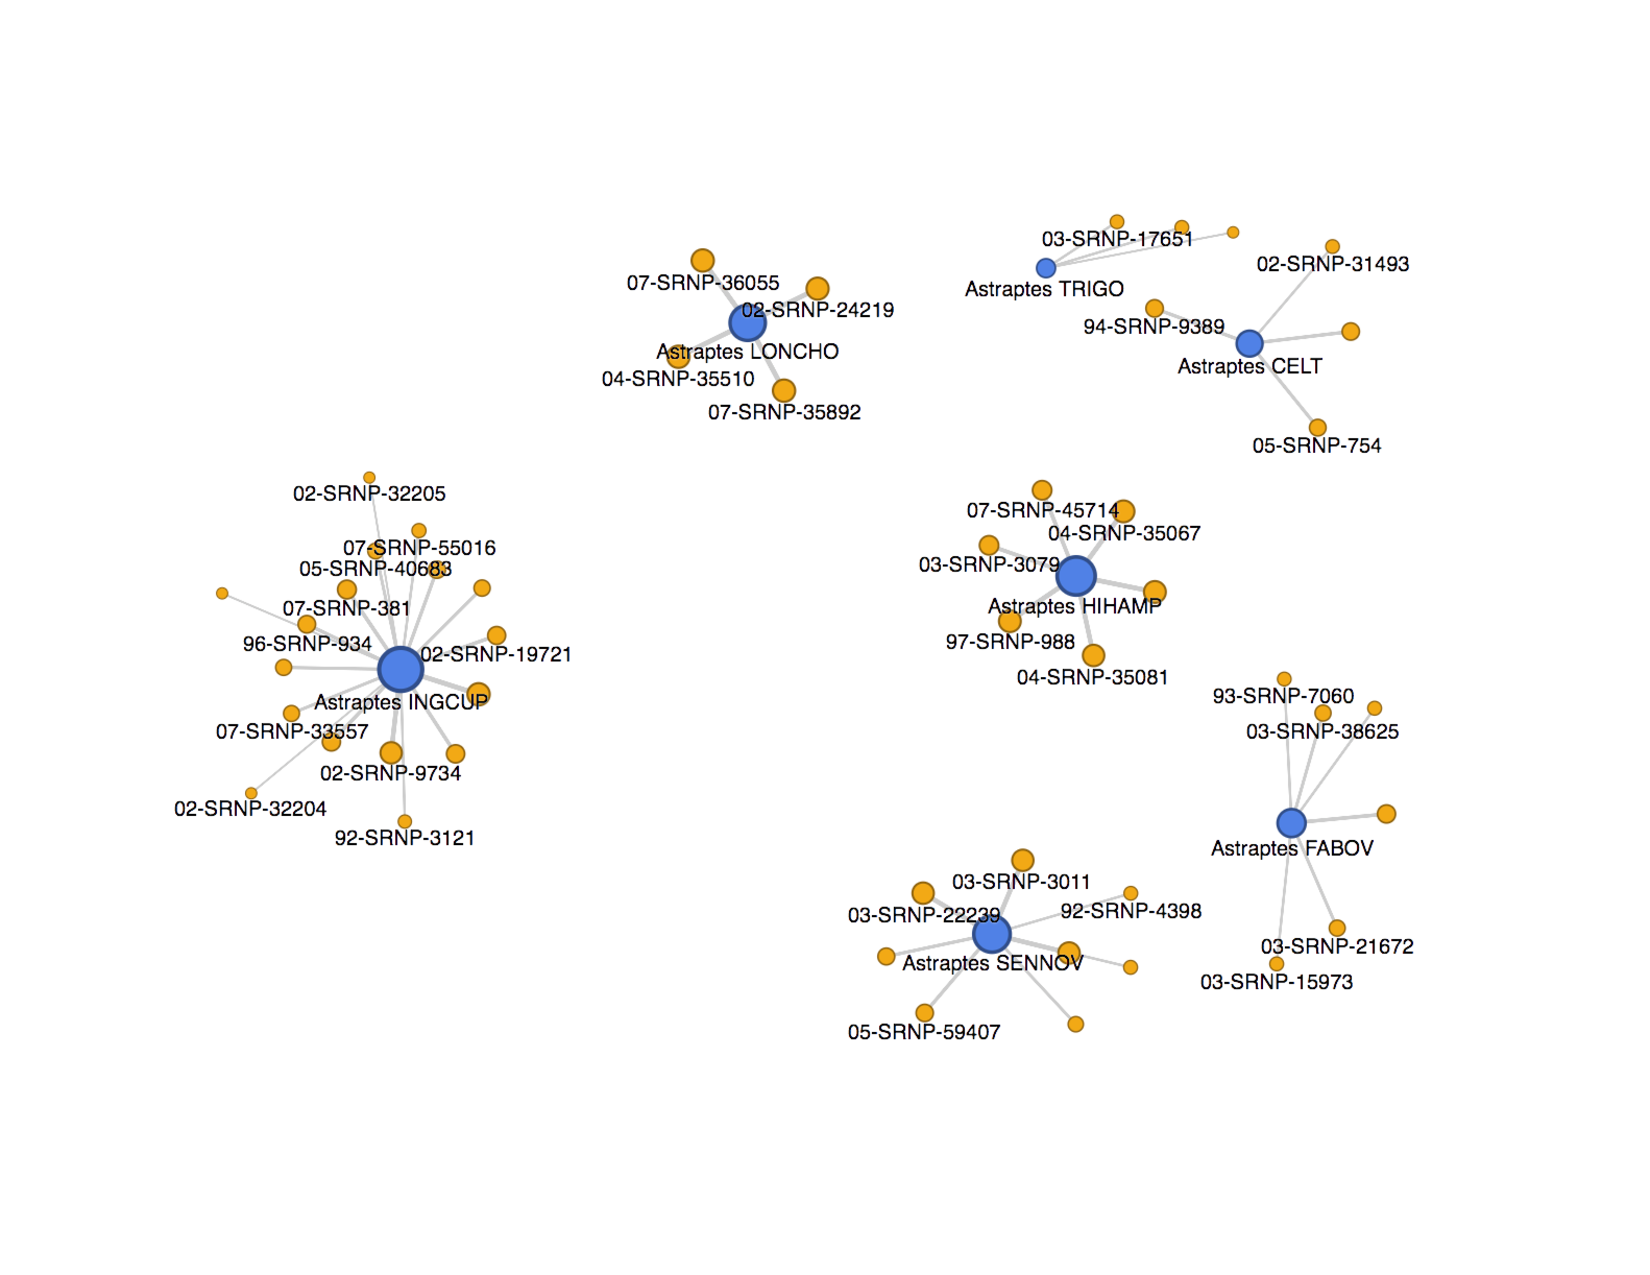
\includegraphics[scale=0.40]{network_graph}
\caption{Exemplo de \textit{Network Graph} utilizando Google Charts}
\label{img:network_graph}
\end{figure}
\end{itemize}

Outro ponto importante na criação do \textit{dashboard} é o uso da paleta de cores. Ying Li e Anshul Sheopuri \cite{li_creative_2015} afirmam que:
\begin{quote}
" Uma cor carrega um significado específico, o qual é baseado no significado aprendido ou no significado biológico"
\end{quote}

 A partir desta afirmação, os autores apresentam uma Tabela \ref{table:cor_significado} que mapeia uma mensagem a uma determinada cor. Utilizando-se a tabela, percebe-se que uma combinação de cores para um \textit{dashboard} seria preto e azul por passar uma mensagem de calma, segurança e autoridade.
\begin{table}[H]
\centering
\caption{Mapeamento de Cores e seus Significados}
\label{table:cor_significado}
\begin{tabular}{|ll|}
\hline
\textbf{Mensagem} & \textbf{Cor}                         \\ \hline
Aventura          & Laranja                              \\ \hline
Acessibilidade    & Laranja                              \\ \hline
Autoridade        & Preto                                \\ \hline
Calma             & Azul                                 \\ \hline
Alegria           & Amarelo, Laranja                     \\ \hline
Limpeza           & Azul, Turquesa e Branco              \\ \hline
Criatividade      & Preto e Magenta, Azul Claro, Amarelo \\ \hline
Inovação          & Amarelo, Roxo, Magenta               \\ \hline
Saúde             & Verde, Marrom                        \\ \hline
Paixão            & Vermelho                             \\ \hline
Segurança         & Azul, Marrom, Verde                  \\ \hline
Saudável          & Verde Escuro, Marrom                 \\ \hline
\end{tabular}
\end{table}

Em seu livro, Stephen Few \cite{book_design} analisa uma variedade de \textit{dashboards} dos quais alguns valem ser mencionados. No \textit{dashboard} da Figura \ref{img:dashboard1}, o uso de \textit{radio buttons} permite que seja feita uma seleção em relação ao período, em que se deseja analisar, porém não permite que seja feita uma comparação entre os períodos. Outro ponto a ser destacado é o uso de uma fotografia no painel. Stephen Few chama isso de \textit{chartjunk}, pois a imagem não tem funcionalidade alguma; a não ser a de decorar o painel. Caso contrário, não é adequado o uso dessa prática. 
\graphicspath{{figuras/}}
\begin{figure}[H]
\centering
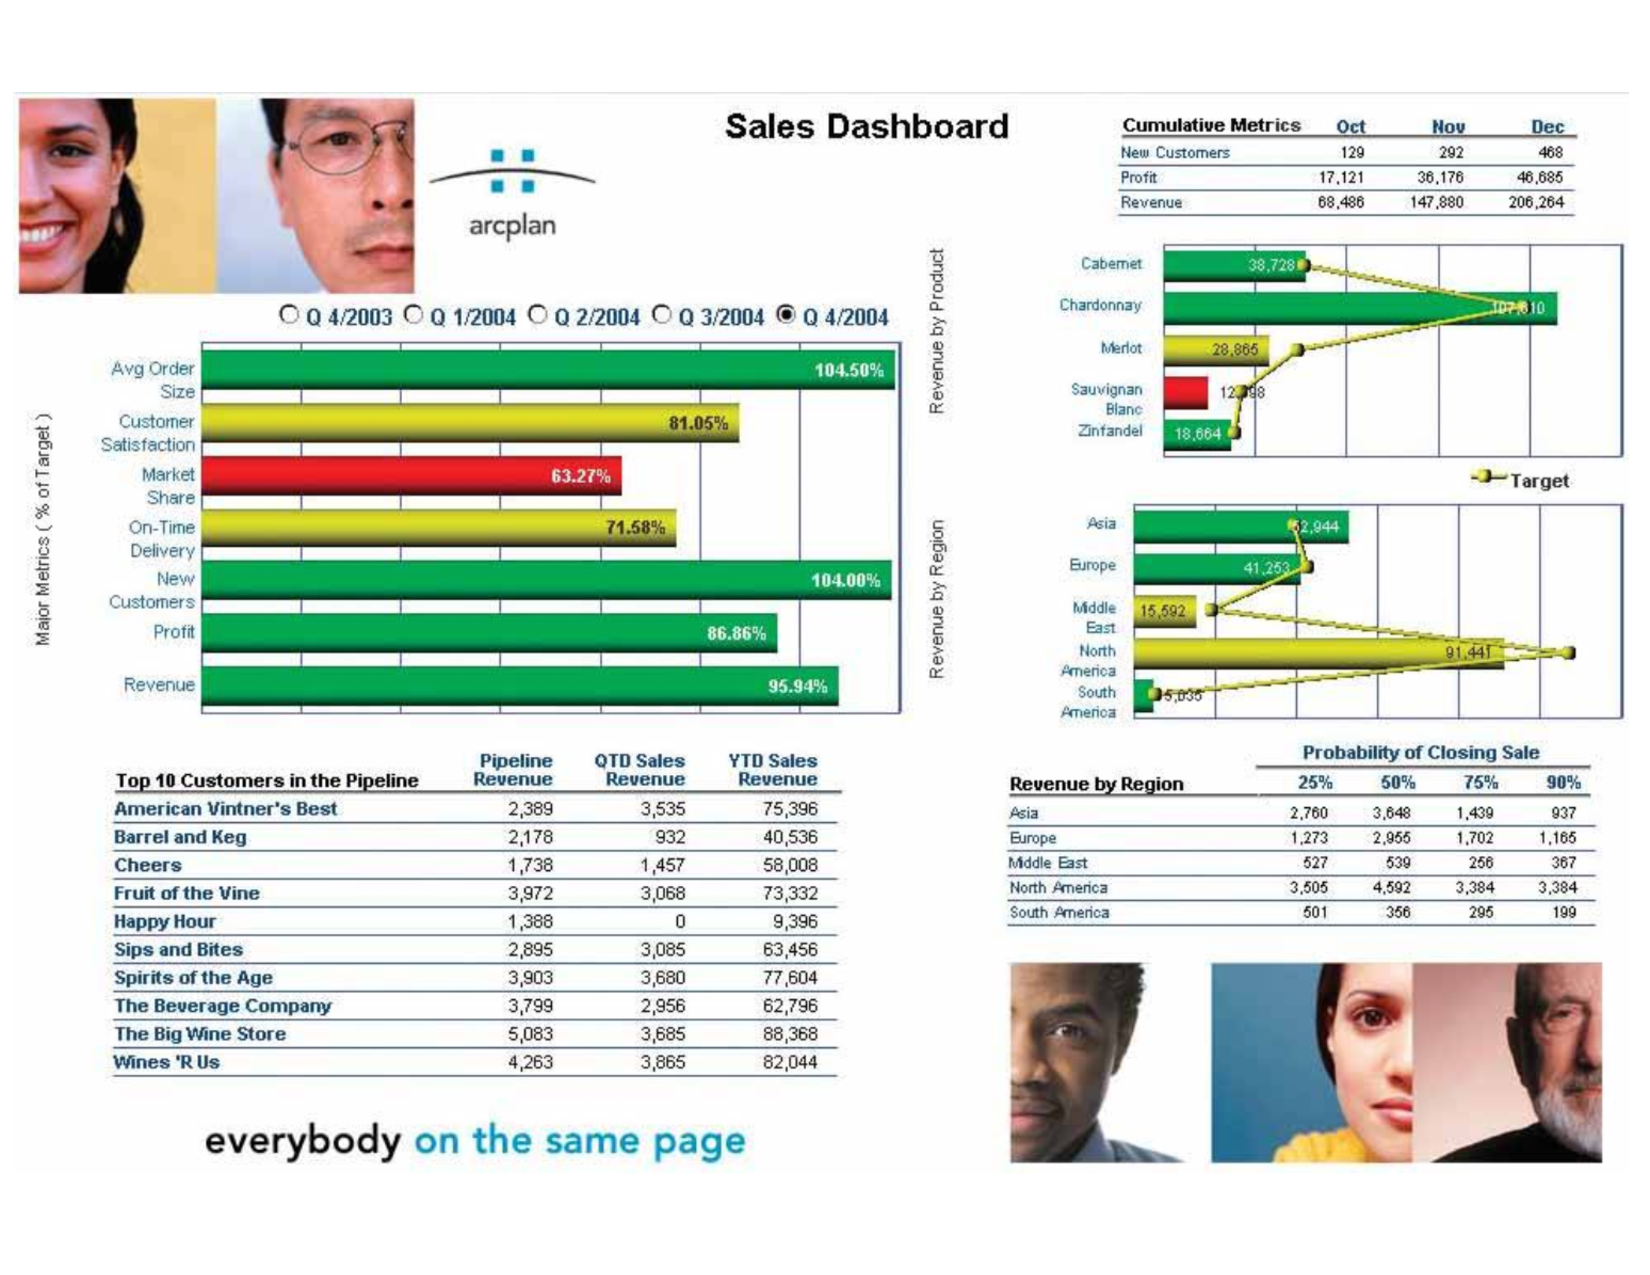
\includegraphics[scale=0.50]{dashboard1}
\caption{Exemplo 1 de \textit{Dashboard} apresentado por Stephen Few. Fonte: \cite{book_design}}
\label{img:dashboard1}
\end{figure}

O segundo \textit{dashboard} (Figura \ref{img:dashboard2}) erra em mostrar as linhas das tabelas e dos gráficos. Essas linhas tiram o foco da informação que se quer transmitir. O uso do gráfico de pizza, neste caso, poderia ser substituído por um gráfico de barras ordenado, que comunicaria a informação de maneira mais eficiente. Um último ponto sobre este \textit{dashboard} é que ele possui muitas cores claras, o que poderia ser substituído por outras tonalidades de cor que fizessem contraste com a informação mais importante.

\graphicspath{{figuras/}}
\begin{figure}[H]
\centering
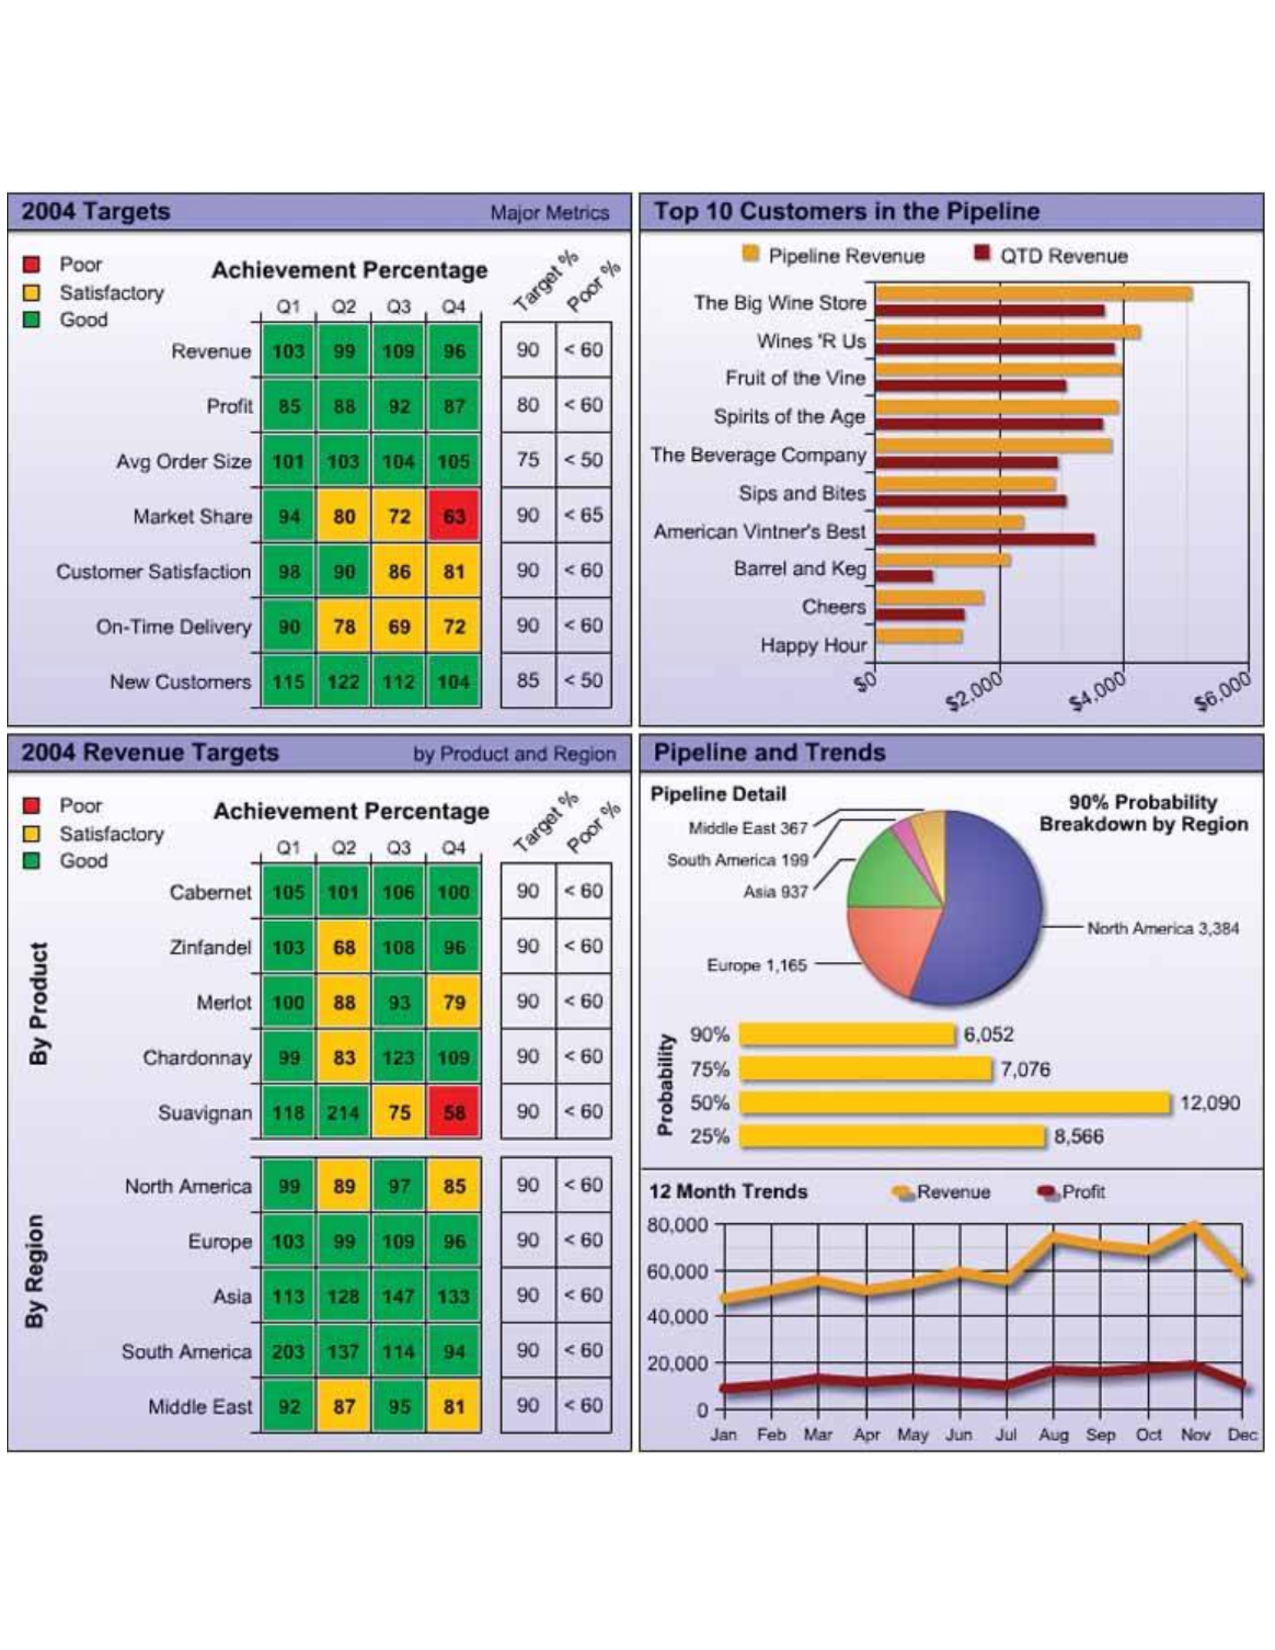
\includegraphics[scale=0.50]{dashboard2}
\caption{Exemplo 2 de \textit{Dashboard} apresentado por Stephen Few. Fonte: \cite{book_design}}
\label{img:dashboard2}
\end{figure}

Por último, o \textit{dashboard} da Figura \ref{img:dashboard3} apresenta ótimas soluções para mostrar a informação quando comparado aos outros dois \textit{dashboards}. O primeiro ponto positivo é o uso do espaço em branco para separar as seções que são apresentadas, o uso da paleta de cores também contribui para esse efeito, as únicas cores encontradas são tons de cinza, verde e dois tons de vermelho. Outro ponto positivo é que toda a informação importante se encontra em um único lugar que é no canto superior esquerdo, onde o leitor começa a leitura.
\graphicspath{{figuras/}}
\begin{figure}[H]
\centering
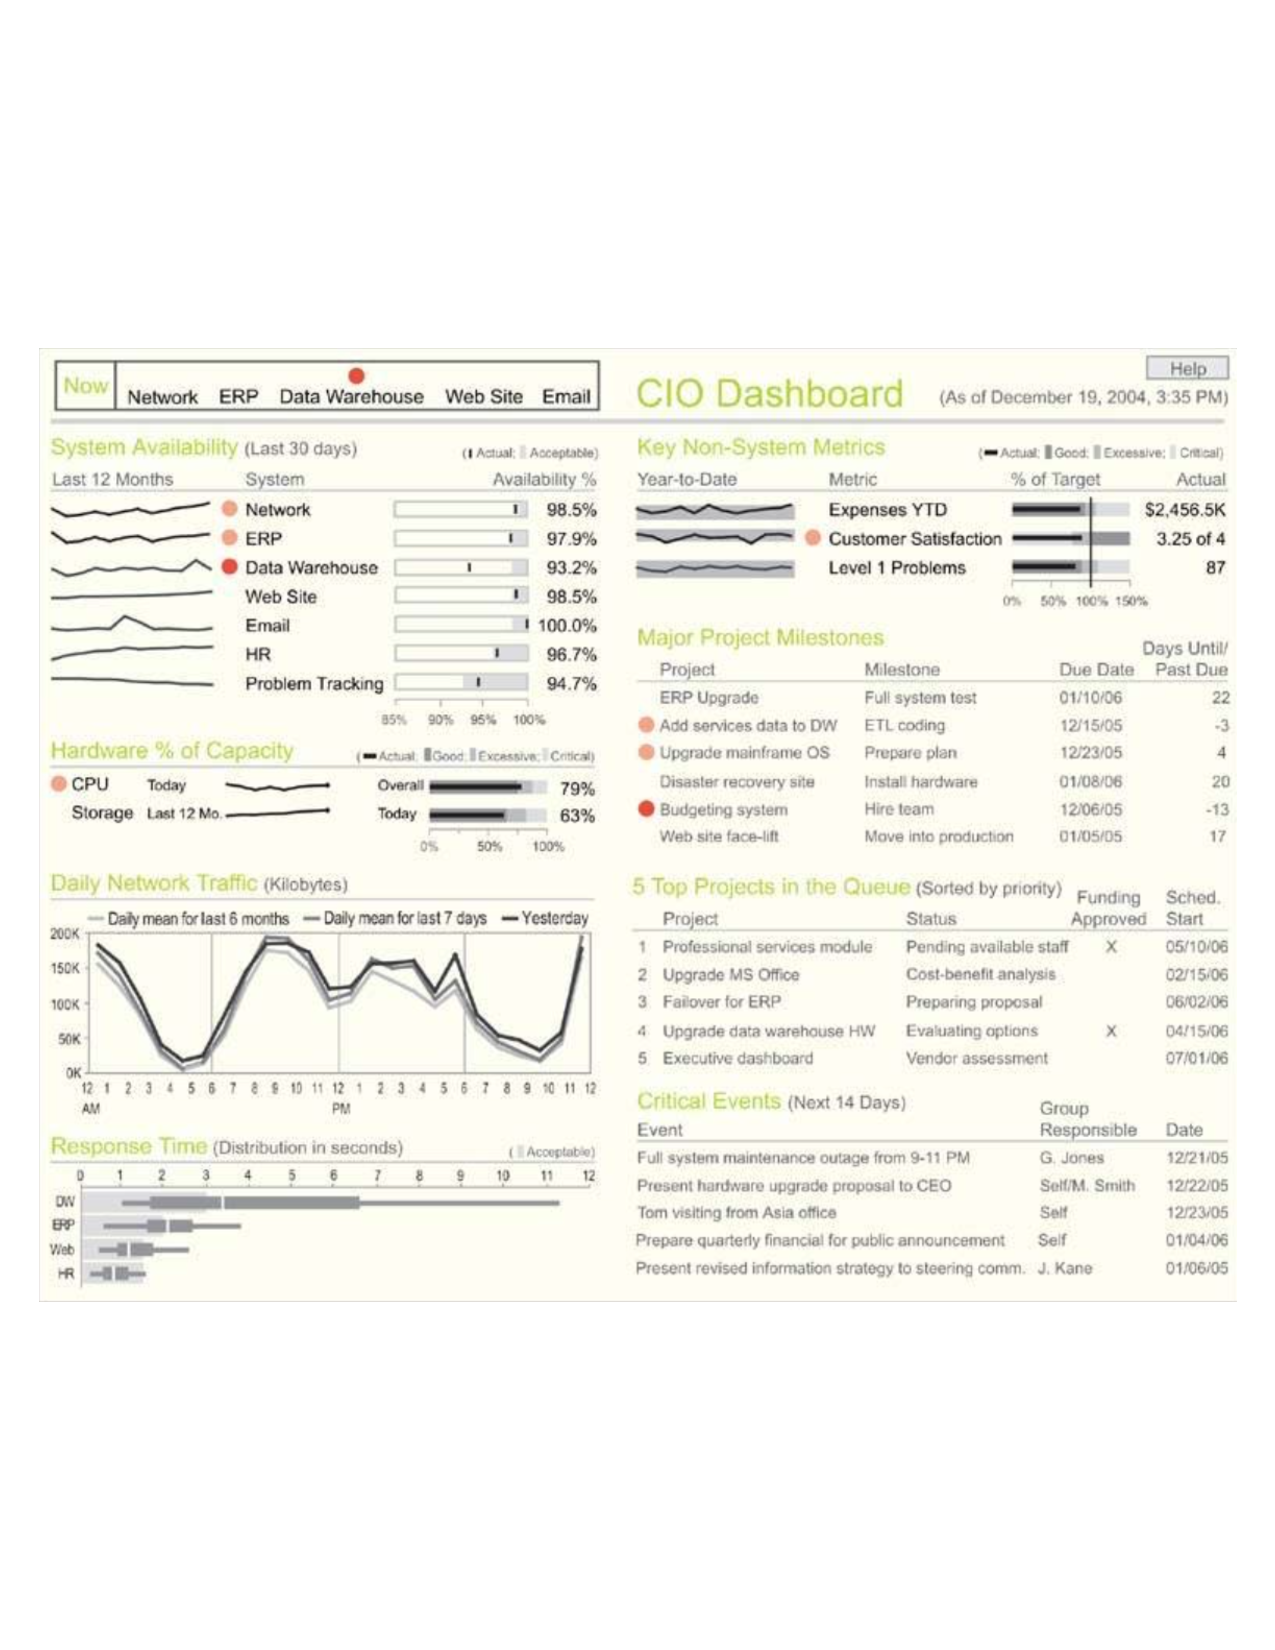
\includegraphics[scale=0.50]{dashboard3}
\caption{Exemplo 3 de \textit{Dashboard} apresentado por Stephen Few. Fonte: \cite{book_design}}
\label{img:dashboard3}
\end{figure}

\section{Questionarios de Avaliação}
Segundo Nunnally \cite{nunnally1978c}, a padronização da medição de indicadores em questionários na área de usabilidade tem como principais vantagens:
\begin{itemize}
\item \textbf{Objetividade:} permite que diferentes pesquisadores tomem como base os mesmos indicadores.
\item \textbf{Replicabilidade:} garante que seja fácil a replicação de estudos feitos por outros pesquisadores, ou até mesmo seus próprios estudos.
\item \textbf{Quantificação:} medições padronizadas permitem que o pesquisador colete resultados com um grau de especificidade maior do que se fossem coletados baseados nos seus próprios julgamentos.
\item \textbf{Economia:} desenvolver medições padronizadas requer um esforço muito grande. Entretanto uma vez que este já foi desenvolvido, o reuso se torna muito mais fácil.
\item \textbf{Comunicação:} se torna fácil a comunicação entre pesquisadores quando se tem um processo de medição  padronizado.
\item \textbf{Generalização Científica:} é o coração do trabalho científico. Padronização é essencial para garantir a generalização dos resultados.

\end{itemize}
 
Sauro \cite{sauro2016quantifying} estabelece quatro questionários de avaliação de usabilidade. A tabela \ref{table:questionarios} apresenta um comparativo entre diferentes questionários. Dentre os questionários abordados escolheu-se o questionário SUS (\textit{Software Usability Scale}) para se realizar a avaliação do projeto. Dois fatores foram levados em consideração para a escolha do questionário, preço e número de perguntas. 

\begin{table}[]
\centering
\caption{Principais Características de Quatro Questionários de Avaliação. Fonte: Adaptado de \cite{sauro2016quantifying}}
\label{table:questionarios}
\begin{tabular}{|ccccc|}
\hline
\multicolumn{1}{|l}{\textbf{Questionário}} & \multicolumn{1}{l}{\textbf{\begin{tabular}[c]{@{}l@{}}Valor da \\ Licença\end{tabular}}} & \multicolumn{1}{l}{\textbf{\begin{tabular}[c]{@{}l@{}}Número de\\  Itens\end{tabular}}} & \multicolumn{1}{l}{\textbf{\begin{tabular}[c]{@{}l@{}}Número de\\  Subescalas\end{tabular}}} & \multicolumn{1}{l|}{\textbf{\begin{tabular}[c]{@{}l@{}}Confiabilidade\\  Global\end{tabular}}} \\ \hline
QUIS                                       & \$50 - 750                                                                               & 27                                                                                      & 5                                                                                            & 0.94                                                                                           \\ \hline
SUMI                                       & 0 - 1000                                                                                & 50                                                                                      & 5                                                                                            & 0.92                                                                                           \\ \hline
PSSUQ                                      & Gratuito                                                                                 & 16                                                                                      & 3                                                                                            & 0.94                                                                                           \\ \hline
SUS                                        & Gratuito                                                                                 & 10                                                                                      & 2                                                                                            & 0.92                                                                                           \\ \hline
\end{tabular}
\end{table}

Brooke \cite{brooke1996sus} define o questionário SUS como sendo uma escala de usabilidade "rápida e suja". O SUS se baseia em um questionário do tipo \textit{"Likert Scale"}, questionários deste tipo apresentam afirmações em que o entrevistado deve julgar o quanto concorda ou discorda da afirmação (no caso do questionário SUS, essa escala varia de 1 a 5).

A escala SU é geralmente utilizada depois que o entrevistado teve a oportunidade de usar o sistema que será avaliado. Deve ser instruído ao entrevistado que se responda imediatamente após ler a pergunta, não se deve pensar muito na resposta pois acaba induzindo o resultado. Todos os itens devem ser marcados e caso o entrevistado não saiba responder um item em particular deve-se marcar o ponto ao centro da escala.

Para calcular o resultado do questionário SUS deve-se somar os valores atribuídos em cada item, sendo que os itens 1,3,5,7 e 9 devem ser subtraídos 1 do valor aferido no questionário (X-1), e nos itens 2,4,6,8 e 10 deve ser subtraído de 5 o valor aferido no questionário (5-X). Feito a soma deve-se multiplicar o resultado obtido 2,5. A escala do Questionário SUS varia de 0 até 100.


\section{Personas}
O método Personas foi criado para ser utilizado no desenvolvimento de soluções de TI, contudo a técnica se tornou comum em outras áreas como desenvolvimento de produtos e na área de \textit{marketing}. Personas são abstrações de um grupo de consumidores reais que dividem um conjunto de características e necessidades em comum \cite{pruitt2010persona}. Personas não podem ser confundidas com estereótipos de uma pessoa. O principal aspecto da descrição de uma persona é que não se deve olhar para toda as características da pessoa em destaque, mas somente para as características relevantes ao contexto.

Uma persona deve ser descrita em forma de narrativa. Segundo Cooper \cite{maness2008using} a descrição em forma de narrativa tem dois objetivos principais, fazer com que a persona se parece com uma pessoa real e prover uma história que expresse as necessidades da persona no contexto do produto que está sendo criado. A narrativa de uma persona começa com a descrição do tipo de indivíduo que aquela persona representa, são detalhados, gostos, costumes, profissão, características físicas. Feito isso, são detalhadas as necessidades específicas daquela persona, são especificados quais são seus objetivos e metas relacionados com o contexto. Estas são as mesmas necessidades que seriam encontradas em um documento de requisitos, contudo estão escritas em forma de narrativa e associadas a uma persona específica \cite{manning2003power}.

Supondo que se queira criar um site de compra de passagens, um exemplo de persona seria: 

Bruce Wayne tem 50 anos, é casado com Diana Prince. Bruce é  um bibliotecário que trabalha na Biblioteca de Gotham City. Uma vez por ano Bruce tira férias de 30 dias para viajar com Diana. Todas as vezes que Bruce viaja ele compra as passagens e reserva o hotel em agências de viagem especializadas. Bruce tem preferência por viajar para lugares com clima frio e que não sejam muito procurados por turistas. Em sua última viagem, Bruce teve um desentendimento com o seu gerente de viagens e por isso quer comprar as passagens e reservar o hotel de maneira que não seja necessário ter que ir a uma agência. Bruce vai comprar as passagens e reservar o hotel através de um celular antigo.

Através do exemplo acima, é possível deduzir um dos públicos alvos do site. Analisando o perfil de Bruce, percebe-se que um possível publico seria adultos com idade próxima aos 50 anos e que são casados. Sabe-se que algumas das funcionalidades do site seriam: ter uma área para compra de passagens e outra para reserva em hotéis. Percebe-se também que o site em questão deve ser responsivo a plataforma em que e apresentado.  


\section{Resumo do Capítulo}

Para que se possa terceirizar o desenvolvimento de software dentro de Órgãos Públicos, algumas regras são necessárias. Entre elas, a de que a empresa vencedora do pregão, a qual irá dispor do direito de produzir o software, entregue o mesmo com qualidade. No edital de contratação, são estabelecidos critérios de qualidade para que o software entregue seja aceito. Estes critérios de qualidade tem sua fundamentação baseada em princípios estabelecidos pela Norma SQuaRE, quanto à categoria de manutenibilidade. Essa categoria é fundamental na contratação de software, pois permite saber o quão manutenível é o software que está sendo contratado. O processo de manutenção de software está intimamente ligado a esta métrica, uma vez que quanto maior a manutenibilidade do software, menos esforço, tempo e dinheiro são gastos nesta etapa. Para definir o grau de manutenibilidade, são apresentadas suítes de métricas que avaliam conceitos específicos do software para validar se o software entregue pela terceirizada é passível de manutenção ou não. Neste trabalho, são apresentadas as métricas presentes no software SonarQube e Codacy. 

Aprendizagem de máquina tem por objetivo auxiliar o computador na tomada de decisões. Para acompanhar a evolução da entrega e se todos os requisitos de análise estática do código estão sendo cumpridos, uma solução seria a utilização de um \textit{dashboard} para acompanhar o desenvolvimento do software a ser entregue. Para isso, faz-se necessário o aprendizado de técnicas de visualização da informação e de conceitos para criação de um \textit{dashboard} efetivo. Ao fim do capítulo é apresentado o SUS que é um questionário de avaliação para avaliar o grau de usabilidade de um sistema.